\documentclass[11pt]{article}
\usepackage[utf8]{inputenc}
\usepackage[margin=1in]{geometry}
\usepackage{amsmath,amssymb,amsthm,mathtools}
\usepackage{booktabs,longtable,array}
\usepackage{microtype}
\usepackage{fancyvrb,multicol}
\usepackage{tikz}
\usetikzlibrary{arrows.meta,calc,positioning}
\usepackage[hidelinks]{hyperref}
\pdfinfoomitdate=1
\pdftrailerid{}
\pdfsuppressptexinfo=15
\hypersetup{
  pdfauthor={OpenAI},
  pdftitle={The critical dimension for one-phase Bernoulli minimizers},
  pdfsubject={The critical dimension of the one-phase Bernoulli problem}
}
\newcommand{\R}{\mathbb R}
\DeclareMathOperator{\tr}{tr}
\DeclareMathOperator{\diver}{div}
\DeclareMathOperator{\Id}{Id}
\DeclareMathOperator{\Sym}{Sym}
\DeclareMathOperator{\STF}{STF}
\DeclareMathOperator{\supp}{supp}
\DeclareMathOperator{\rank}{rank}
\newtheorem{theorem}{Theorem}[section]
\newtheorem{lemma}[theorem]{Lemma}
\newtheorem{proposition}[theorem]{Proposition}
\newtheorem{corollary}[theorem]{Corollary}
\theoremstyle{definition}
\newtheorem{definition}[theorem]{Definition}
\theoremstyle{remark}
\newtheorem{remark}[theorem]{Remark}
\numberwithin{equation}{section}
\allowdisplaybreaks[1]
\title{The critical dimension for one-phase Bernoulli minimizers}
\author{OpenAI}
\date{September 24, 2026}

\begin{document}
\maketitle
\begin{abstract}
We prove that seven is the critical dimension for the one-phase Bernoulli
problem: every nonzero one-homogeneous global minimizer in dimensions at most
six is flat, while a nonflat one-homogeneous global minimizer exists in
dimension seven. It follows that the interior free boundary of a local
minimizer is smooth in dimensions at most six. In dimension $n\ge7$, its
singular set has Hausdorff dimension at most $n-7$, and this bound is sharp.
In dimension seven, the singular set is locally finite.
\end{abstract}

\section{Introduction}\label{sec:introduction}
For a nonnegative function \(v\in H^1(B)\), where \(B\subset\R^d\) is a ball,
the one-phase Bernoulli energy is
\begin{equation}\label{eq:energy}
  J(v;B)=\int_B\bigl(|\nabla v|^2+\mathbf 1_{\{v>0\}}\bigr)\,dx.
\end{equation}
A nonnegative \(u\in H^1_{\mathrm{loc}}(\R^d)\) is a \emph{global minimizer}
if \(J(u;B)\leq J(v;B)\) for every ball \(B\) and every nonnegative
\(v\in H^1(B)\) with \(v-u\in H^1_0(B)\).
The competitors in these comparisons are arbitrary Sobolev functions with
the prescribed trace.
A function is \emph{one-homogeneous} if \(u(rx)=r u(x)\) for every \(r>0\),
almost everywhere in \(x\).
The nonzero flat solutions are
\[
  u(x)=(x\cdot e)_+,\qquad |e|=1.
\]
Let \(d_*\) be the least dimension containing a nonzero, nonflat,
one-homogeneous global minimizer.

\begin{theorem}\label{thm:main}
Every nonzero one-homogeneous global minimizer of \eqref{eq:energy}
in \(\R^d\), \(1\leq d\leq6\), is flat. There is a nonflat
one-homogeneous global minimizer in \(\R^7\). Consequently,
\[
  d_*=7.
\]
\end{theorem}

A nonnegative $u\in H^1_{\mathrm{loc}}(D)$ is a local minimizer in an open
set $D\subset\R^n$ if it satisfies the same
comparison on every ball compactly contained in $D$. At an interior
free-boundary point $x_0$, a \emph{blowup} is a locally uniform limit of
$u(x_0+rx)/r$ along radii tending to zero. A point is regular if one such
limit is a flat solution, and singular otherwise. Write $\operatorname{Sing}(u)$
for the set of singular points in $D$.

\begin{corollary}[Sharp singular-set bound]\label{cor:singular-set}
Let $n\ge2$, let $D\subset\R^n$ be open, and let $u\in H^1_{\mathrm{loc}}(D)$ be a nonnegative local
minimizer of the one-phase Bernoulli energy in $D$.
Its interior free boundary is smooth outside $\operatorname{Sing}(u)$.
This set is empty when $n\le6$, is locally finite when $n=7$, and satisfies
\[
 \dim_{\mathrm H}\operatorname{Sing}(u)\le n-7\qquad(n\ge7).
\]
For every $n\ge7$, a global minimizer attains this dimension bound.
\end{corollary}

The upper bound is the standard dimension-reduction consequence of the
critical dimension, and sharpness follows by taking Cartesian products of
the De Silva--Jerison cone with Euclidean space. We verify these deductions
in Section~\ref{sec:consequences}.

The variational theory of the one-phase Bernoulli problem begins with
Alt and Caffarelli's existence and regularity theory
\cite{AltCaffarelli1981}.  Weiss's monotonicity formula and dimension
reduction \cite{Weiss1999} connect the singularities of general minimizers
to homogeneous global minimizers; see also
\cite[Theorem~1.4 and Chapters~9--10]{Velichkov2023}.
Thus the first dimension admitting a nonflat minimizing cone determines
both the threshold for singular free boundaries and the codimension
bound furnished by this theory.  Our main result answers positively
the critical-dimension question whether $d_*=7$.

A second strand of the theory passes from weak free boundaries to
classical ones. Caffarelli's Harnack-inequality approach established
regularity for Lipschitz free boundaries \cite{Caffarelli1987}.
De Silva developed a different improvement-of-flatness argument allowing
a nonzero right-hand side \cite[Theorems~1.1--1.2]{DeSilva2011}; this is the approach
presented in the regularity chapters of \cite{Velichkov2023}.
Higher regularity has classical antecedents in Kinderlehrer and Nirenberg
\cite[Theorem~2]{KinderlehrerNirenberg1977}. The version used here, for
Lipschitz viscosity solutions, is due to De Silva, Ferrari and Salsa
\cite[Theorem~1.1 and Corollary~1.2]{DeSilvaFerrariSalsa2019}.
These results make a classification of
homogeneous minimizing blowups applicable to general local minimizers.

As recalled by Jerison and Savin \cite[Introduction]{JerisonSavin2015},
the dimension-three rigidity result for stable homogeneous solutions
with smooth cross-section is due to Caffarelli, Jerison and Kenig
\cite{CaffarelliJerisonKenig2004}.
Jerison and Savin proved that stable homogeneous solutions with smooth
cross-section are flat in dimensions at most four
\cite[Theorem~1.1]{JerisonSavin2015}; their regularity consequence for
minimizers \cite[Corollary~1.2]{JerisonSavin2015} gives $d_*\geq5$.
Their argument constructs functions of the Hessian satisfying
inequalities for the linearized free-boundary problem.  In the other
direction, De Silva and Jerison constructed a nonflat homogeneous
global minimizer in dimension seven
\cite[Theorem~1.1]{DeSilvaJerison2009}, proving $d_*\leq7$.
The minimizing property in that construction is with respect to all
Sobolev competitors with the prescribed boundary trace. Firester,
Tsiamis and Wang also construct further symmetric minimizing
one-phase cones, including a second example in dimension seven
\cite[Theorem~1.4]{FiresterTsiamisWang2026Capillary}.

Recent work further describes cones with symmetry.  Firester, Tsiamis
and Wang \cite[Theorem~1.1]{FiresterTsiamisWang2026} prove that their
cohomogeneity-one cones with $O(n-k)\times O(k)$ symmetry,
$1\leq k\leq n-2$, are unstable for $n\leq6$ and strictly stable for
$n\geq7$.  The exclusion proved here applies to globally
minimizing cones without a symmetry assumption.

Cone classification also differs from rigidity of arbitrary entire
stable solutions. Fern\'andez-Real and Serra prove that every global
classical stable solution in dimension four is one-dimensional
\cite[Theorem~1.1]{FernandezRealSerra2026}. Their result removes homogeneity in
that dimension.

For an admissible increasing family of nonnegative boundary data,
Fern\'andez-Real and Yu prove regularity through dimension six for
almost every parameter
\cite[Assumption~1 and Theorem~1.3]{FernandezRealYu2025}.
This is a generic-data result: the increase is required at a fixed linear
rate on the positive set of the smaller boundary datum.

\paragraph{The obstacle and the proof strategy.}
The stability inequality compares the Dirichlet energy of a test function
with a curvature term on the free boundary.  The use of the harmonic Hessian has a geometric precedent in Simons's
second-fundamental-form argument for minimal cones \cite[Section~6.1]{Simons1968},
a connection developed explicitly by Jerison and Savin. A natural
Bernoulli test is a power of the Hessian norm. Jerison and Savin explain why
this unweighted choice does not give a uniform instability criterion in
dimensions four through six: the interior and boundary estimates impose
different restrictions on the power, and their sharp configurations need
not agree
\cite[Section~3.2]{JerisonSavin2015}.  Their four-dimensional argument
uses a more refined function of the Hessian eigenvalues
\cite[Section~4]{JerisonSavin2015}.

Our proof uses the normalized shape of the Hessian to construct both
a scalar test and a separate vector field whose divergence controls
the test's energy.  The two constructions are chosen together, so
the interior and boundary estimates retain the same tensor data.
The proof has three stages.

First, suppose the first nonflat minimizing cone occurs in dimension
five or six.  Blowups away from its vertex reduce the dimension and
are therefore flat.  Regularity theory makes each component of its
spherical positive set smooth, and at least one component has
nonzero Hessian.  A five-dimensional cone can be made independent
of one extra coordinate without losing minimality.  Its spherical
link then has precisely two exceptional tips.  Thus both possible
dimensions lead to a domain $\Omega\subset S^5$ with a smooth
regular boundary and, possibly, these two tips
(Section~\ref{sec:reductions}).

Second, let $g$ be the restriction of the resulting cone to the sphere,
and set $T=\nabla^2g+g\Id$ and $w=|T|$.  Where $w>0$, we construct
a positive scalar $h$ from $w$, the normalized tensor $T/w$, $g$,
and $\nabla g$, and
a vector field $Z$ from the same data and $\nabla T/w$.  The target
inequalities are
\[
  \diver Z\ge |\nabla h|^2+4h^2+\epsilon_*w^{2a},
  \qquad N\cdot Z+Hh^2\ge0,
\]
where $a\in(1/2,1)$ is fixed, $\epsilon_*>0$, $N$ points into $\Omega$, and
$H=-T(N,N)$.  Spherical stability supplies the reverse integrated
comparison between the test's energy and its boundary curvature term.
The extra positive mass $\epsilon_*w^{2a}$ will give the contradiction.
The geometry and stability inequality are developed in
Section~\ref{sec:geometry}. We then state the universal tensor inequality
and derive the two geometric comparisons; the full exact verification
follows in Section~\ref{sec:certificate-proof}.

Two cancellations make this construction possible.  A Laplacian
contraction and an antisymmetric curvature contraction eliminate
fourth derivatives from $\diver Z$.  At the boundary, reflection
in the normal direction removes the derivative components not
determined by the boundary conditions.  The remaining inequalities
involve only finitely many normalized tensors.  We prove them by
weighted sums of tensor squares and exact rational remainder bounds,
with all coefficients and contraction conventions supplied in
Appendix~\ref{app:tables}.

Finally, neither the normalized Hessian nor its derivatives are defined
at $w=0$, and suspension introduces singular tips.  These sets cannot
be discarded without an estimate.  A regularized Bochner identity
gives an integrable weight controlling the derivatives near every
Hessian zero.  The explicit suspension formulas give an integrable
power of the distance parameter at both tips.  Smooth product
cutoffs therefore remove both obstructions and make all error terms
vanish.  Section~\ref{sec:cutoffs} completes the stability
contradiction.


\paragraph{Organization and conventions.}
Section~\ref{sec:reductions} reduces a hypothetical first nonflat minimizer
to a smooth spherical component in dimension six, allowing two suspension
tips. Section~\ref{sec:geometry} derives the tensor identities and the
stability inequality. Section~\ref{sec:certificate} states the universal
algebraic estimate, and Section~\ref{sec:flux} derives the pointwise
geometric comparison from it. Section~\ref{sec:certificate-proof} gives
the complete exact verification; Section~\ref{sec:cutoffs} then removes
the cutoffs to obtain the contradiction. Section~\ref{sec:consequences}
gives the regularity and sharpness consequences.
Appendix~\ref{app:tables} gives all coefficient data.
All tensor norms and contractions use orthonormal frames. Repeated indices
are summed, \(\Delta=\tr\nabla^2\), and a boundary normal denoted by \(N\)
points into the positive phase. The curvature \(H=-T(N,N)\) used below is
not divided by the dimension of the boundary.

\section{Reduction to a smooth link and its suspension}\label{red:section}\label{sec:reductions}

We first record the consequences of energy minimality needed to put the
argument on a smooth spherical domain.  Throughout Section~\ref{sec:reductions}, a minimizer
has the full ballwise Sobolev comparison property defined in
Section~\ref{sec:introduction}.

\subsection{The regularity inputs}\label{red:regularity-inputs}

The ballwise convention also gives comparison on every bounded open set
$O\Subset\R^d$: extend an $H^1_0(O)$ competitor difference by zero into a ball
containing $\overline O$, apply minimality there, and cancel the energy outside
$O$.  Conversely, comparison on bounded open sets includes comparison on
balls.  It is even enough to have comparison against \emph{arbitrary}
admissible competitors in every origin-centered ball, by the same extension
argument.  There is no restriction to homogeneous competitors.

The convention that competitors are nonnegative makes no difference to the
standard one-phase results.  If $v-u\in H^1_0(O)$ and $u\geq0$, then
$v_+-u\in H^1_0(O)$ and
\[
 \int_O\bigl(|\nabla v_+|^2+\mathbf 1_{\{v_+>0\}}\bigr)
 \leq
 \int_O\bigl(|\nabla v|^2+\mathbf 1_{\{v>0\}}\bigr).
\]
For completeness, the assertion about $H^1_0(O)$ follows by approximating
$v-u$ in $H^1$ by compactly supported smooth functions and applying the
continuity of positive-part truncation in $H^1$; the truncated differences
in the approximation have compact support in $O$.

\begin{proposition}[Regularity and blowups of minimizers]\label{red:regularity}
Let $d\geq2$ and let $u\geq0$ be a local minimizer of the one-phase energy
with volume coefficient $1$ in an open set $D\subset\R^d$.
\begin{enumerate}
\renewcommand{\labelenumi}{\textup{(\roman{enumi})}}
\item There is a locally Lipschitz representative of $u$, and it is harmonic
in $\{u>0\}$.
\item If $x_0\in D\cap\partial\{u>0\}$, every sequence $r_j\downarrow0$
has a subsequence for which
\begin{equation}\label{red:blowup-sequence}
 u_{x_0,r_j}(y):=\frac{u(x_0+r_jy)}{r_j}\longrightarrow U(y)
\end{equation}
locally uniformly in $\R^d$.  The limit is a nonzero, nonnegative,
one-homogeneous global minimizer.  Along a further subsequence the convergence
is strong in $H^1_{\mathrm{loc}}$, and the positivity indicators converge in
$L^1_{\mathrm{loc}}$.
\item If one such limit equals $(y\cdot e)_+$ with $|e|=1$, then near
$x_0$ the free boundary is a smooth hypersurface and $\{u>0\}$ is exactly
one of its sides.  The function $u$ is smooth up to that hypersurface from
the positive side, and
\begin{equation}\label{red:bernoulli}
 u=0,\qquad \nabla u=N_E
 \quad\hbox{on the free boundary},
\end{equation}
where $N_E$ is the Euclidean unit normal pointing into $\{u>0\}$.
\end{enumerate}
\end{proposition}

\begin{proof}[Sources and applicability]
We use the constant-coefficient theory with $\Lambda=1$ in
\cite{Velichkov2023}.  For each ball $B\Subset D$, the restriction of $u$
to $B$ minimizes against every $H^1_0(B)$ competitor difference.
Zero extension of differences therefore gives comparison on every
$O\Subset B$, as required by Definitions~2.11--2.12 there. We apply the
local results inside such balls. For global minimizers, the containing-ball
argument above gives the comparison convention on all bounded open sets.
Local Lipschitz continuity is Theorem~3.1. Harmonicity also follows
directly: for a smooth test supported compactly in the positive phase, both
signs of a sufficiently small additive variation preserve that phase, so the
Dirichlet first variation vanishes.

The Lipschitz bound and $u(x_0)=0$ give locally uniform compactness of the
rescalings.  Proposition~4.1 gives
$\sup_{B_r(x_0)}u\geq\kappa r$ for small $r$, with $\kappa>0$, so a limit
cannot vanish identically.  Proposition~6.2 gives strong Sobolev and
positivity-indicator convergence and the full minimizing property of the
limit; Proposition~9.12 gives its one-homogeneity.  All these statements can
be applied in a bounded ball compactly contained in $D$ before taking the
rescalings.  In particular, the assertion about minimality is the minimizing
compactness result, including the volume term.

Definition~6.10 and Corollary~8.2, with the one-sided graph conclusion in
Theorem~8.1, give a $C^{1,\alpha}$ regular neighborhood from a single
half-space blowup.  Proposition~7.1 supplies the viscosity Bernoulli condition.

To justify all subsequent boundary derivatives, use
\cite[Theorem~1.1 and Corollary~1.2]{DeSilvaFerrariSalsa2019} with
$f_+=f_-=0$ and $G(b)=1+b$.  We check the two-phase viscosity condition
of \cite[Definition~7.1]{DeSilvaFerrariSalsa2014} when $u\geq0$.
Let $v$ be a comparison touching $u$ at a free-boundary
point $x_0$, with a $C^2$ interface and $C^2$ branches having nonnegative
normal slopes $a$ and $b$ on its positive and negative sides.  If $v$ touches
from below, then $v_+\leq u$ in a neighborhood.  For $a>0$, extend its
positive branch to a signed $C^2$ function $\phi$, negative just across
the interface; then $\phi\leq u$ and touches at $x_0$.  The one-phase
condition gives $a\leq1\leq G(b)$; the case $a=0$ is immediate.  If $v$
touches from above, the neighborhood inequality $v\geq u\geq0$ forces
$v=u=0$ throughout its nonpositive side, so $b=0$.  A $C^2$ extension
$\phi$ of its positive branch satisfies $\phi_+\geq u$ on both sides
and touches at $x_0$.  Thus the one-phase condition gives $a\geq1=G(0)$.
These uses of the one-phase condition are justified by
\cite[Definition~7.6 and Proposition~7.1]{Velichkov2023}: to meet its
smooth-test convention, replace each $C^2$ extension by its quadratic
Taylor polynomial minus, respectively plus, $\varepsilon|x-x_0|^2$.
For any $\varepsilon>0$, these are smooth lower and upper supports in a
sufficiently small neighborhood, with the same contact value and gradient.

The interior equations hold because $u$ is harmonic where positive and
identically zero on the interior of its zero set.  The function $G$ is smooth,
strictly increasing and unbounded, with $G(0)=1$; the cited results allow
the negative phase to vanish.  The preceding $C^{1,\alpha}$ one-sided graph
satisfies the slab flatness hypothesis after rotation and sufficiently small
dilation, while the local Lipschitz bound is preserved.  Theorem~1.1 gives
$C^{2,\gamma}$ regularity, and Corollary~1.2 gives smoothness.  Local harmonic boundary regularity with zero Dirichlet data
\cite[Theorems~4.30--4.31 and Corollary~4.32]{Hunter2014} then gives
smoothness of $u$ from the positive side. These estimates apply after
flattening a smooth boundary patch and localizing away from its artificial
boundary; iteration and Sobolev embedding give every required derivative.  The Bernoulli condition and nonnegativity give
\eqref{red:bernoulli}.
\end{proof}

As in Section~\ref{sec:introduction}, a free-boundary point is regular
if it has a half-space blowup and singular otherwise.  Proposition~\ref{red:regularity} explains the
geometric meaning of regularity.  Conversely, a smooth one-sided free
boundary with \eqref{red:bernoulli} has a half-space blowup by its first-order
Taylor expansion.  We henceforth use the continuous representative of a
minimizer.  If it is one-homogeneous almost everywhere, it is one-homogeneous
everywhere: for each fixed $r>0$, both sides of $u(rx)=ru(x)$ are continuous
and agree almost everywhere.

\subsection{Dimension reduction at a nonzero point}\label{red:dimension-reduction}

The next two lemmas give the dimension-reduction steps explicitly;
compare \cite[Lemmas~10.9--10.10]{Velichkov2023}.

\begin{lemma}[Translation invariance of an off-origin blowup]\label{red:translation}
Let $u$ be a one-homogeneous global minimizer, let
$0\ne x_0\in\partial\{u>0\}$, and let $U$ be any limit in
\eqref{red:blowup-sequence}.  Then
\[
 U(y+t x_0)=U(y)\qquad(y\in\R^d,\ t\in\R).
\]
\end{lemma}

\begin{proof}
Write $u_r=u_{x_0,r}$.  For fixed $t\in\R$ and small $r>0$, set
$r'=r/(1+rt)>0$.  Homogeneity gives the exact identity
\begin{equation}\label{red:rescaling-identity}
 u_r(y+t x_0)
 =\frac{u\bigl((1+rt)(x_0+r'y)\bigr)}r
 =u_{r'}(y).
\end{equation}
Let $L$ be a Lipschitz constant for $u$ on a fixed neighborhood of $x_0$.
Since $u(x_0)=0$, for $|y|\leq M$ and small $r$,
\begin{align*}
 |u_{r'}(y)-u_r(y)|
 &\leq\frac{L|r-r'|M}{r'}
       +LrM\left|\frac1{r'}-\frac1r\right|\\
 &=2LM\frac{|r-r'|}{r'}=2LM|t|r.
\end{align*}
Thus the $r'$ rescalings along the same chosen sequence have the same
locally uniform limit as the $r$ rescalings.  Passing to that limit in
\eqref{red:rescaling-identity} proves the assertion for every fixed $y,t$.
No uniqueness of blowups is required.
\end{proof}

\begin{lemma}[Minimality of a translation-invariant factor]\label{red:factor-minimality}
Suppose $U(y,s)=v(y)$ is a global minimizer in
$\R^k\times\R$, where $v\geq0$ belongs to $H^1_{\mathrm{loc}}(\R^k)$.
Then $v$ is a global minimizer in $\R^k$.
\end{lemma}

\begin{proof}
Suppose that a ball $B\subset\R^k$ admits a nonnegative
$q\in H^1(B)$ with $q-v\in H^1_0(B)$ and
\[
 J(v;B)-J(q;B)=\delta>0.
\]
Let $\psi$ be the zero extension of $q-v$.  For $L>1$, choose
$\eta_L:\R\to[0,1]$ equal to $1$ on $[-L,L]$, equal to $0$ outside
$[-L-1,L+1]$, and linear on each intervening interval.  Define
\[
 V_L(y,s)=U(y,s)+\eta_L(s)\psi(y).
\]
This function is nonnegative: on $B\times\R$ it is the convex combination
$(1-\eta_L)v+\eta_Lq$.  Its difference from $U$ belongs to $H^1$ and has
compact support in a sufficiently large ball $\mathcal B_L\subset\R^{k+1}$,
so it belongs to $H^1_0(\mathcal B_L)$.

The energy difference on $B\times[-L,L]$ is $-2L\delta$.  On either
transition cylinder, convexity gives
\[
 |\nabla_y V_L|^2\leq(1-\eta_L)|\nabla v|^2+\eta_L|\nabla q|^2,
 \qquad |\partial_sV_L|^2\leq|q-v|^2.
\]
The difference of the positivity indicators is at most $1$.  Hence the
sum of the two transition contributions is bounded above by
\[
 C=2\int_B\bigl(|\nabla q|^2+|q-v|^2+1\bigr),
\]
independently of $L$.  Outside these three cylinders the energy is unchanged.
Thus
\[
 J(V_L;\mathcal B_L)-J(U;\mathcal B_L)\leq-2L\delta+C<0
\]
for large $L$, contradicting minimality of $U$.
\end{proof}

In dimension one, every nonnegative one-homogeneous Sobolev function
has the form $u(x)=b_+x_++b_-(-x)_+$ with $b_+,b_-\ge0$.
If both slopes are positive, a nonnegative smooth bump $\phi$ supported
in $(-R,R)$ with $\phi(0)>0$ preserves positivity volume and gives
\[
 J(u+\tau\phi;(-R,R))-J(u;(-R,R))
 =-2\tau(b_++b_-)\phi(0)+\tau^2\int_{-R}^R|\phi'|^2<0
\]
for small $\tau>0$. Thus a nonzero minimizing cone has just one positive
slope. After reflection write $u(x)=b x_+$, $b>0$.
The competitors $v_t(x)=bR(x-t)_+/(R-t)$ on $(-R,R)$, $|t|<R$,
have the same trace and energy $b^2R^2/(R-t)+(R-t)$.
Its derivative at the minimizing parameter $t=0$ is $b^2-1=0$,
so $b=1$. This proves flatness in dimension one directly.

The lower-dimensional classification of Jerison--Savin
\cite[Theorem~1.1 and Corollary~1.2]{JerisonSavin2015} and the
dimension-seven minimizing example of De Silva--Jerison
\cite[Theorem~1.1]{DeSilvaJerison2009} give $5\leq d_*\leq7$.
De Silva--Jerison's Theorem~1.1 uses the same functional and arbitrary
ballwise Dirichlet competitors.  For the exclusion argument, suppose from
now on that
\begin{equation}\label{red:first-dimension}
 d=d_*\in\{5,6\},
\end{equation}
and fix a nonzero nonflat one-homogeneous global minimizer $u$ in $\R^d$.

\begin{proposition}[Smooth original link]\label{red:original-link}
Every point of $\partial\{u>0\}\setminus\{0\}$ is regular.  Put
$m_o=d-1$ and $g_o=u|_{S^{m_o}}$.  The set $\{g_o>0\}$ is nonempty and
proper, has finitely many connected components, and their closures are
pairwise disjoint compact smooth manifolds with boundary.  On each such
component $\Omega_o$, the restriction of $g_o$ is smooth up to the boundary
from within $\Omega_o$ and satisfies
\begin{equation}\label{red:link-equations}
 \Delta_{S^{m_o}}g_o=-m_o g_o\quad\hbox{in }\Omega_o,
 \qquad g_o=0,\quad \nabla_{S^{m_o}}g_o=N_o
       \quad\hbox{on }\partial\Omega_o,
\end{equation}
where $N_o$ is the inward spherical unit normal.  In particular,
$\partial\Omega_o\ne\varnothing$.
\end{proposition}

\begin{proof}
At a nonzero free-boundary point $x_0$, choose a blowup $U$ from
Proposition~\ref{red:regularity}.  By Lemma~\ref{red:translation}, in
orthogonal coordinates $\R^d=x_0^\perp\times\R$ it has the form
$U(y,s)=v(y)$.  The factor $v$ is locally Lipschitz, nonnegative, nonzero
and one-homogeneous.  Lemma~\ref{red:factor-minimality} shows that it is a
global minimizer.  Since its dimension is $d-1<d_*$, it is flat.  Therefore
$U$ itself is a half-space solution, and Proposition~\ref{red:regularity}
makes $x_0$ regular.

The spherical positive set is nonempty by nontriviality.  The polar-coordinate
formula for the Euclidean Laplacian of $u(ry)=r g_o(y)$ gives
\begin{equation}\label{red:polar-laplacian}
 \Delta_{\R^d}u(ry)=r^{-1}
       \bigl(\Delta_{S^{m_o}}g_o(y)+m_o g_o(y)\bigr)
\end{equation}
in the positive phase.  If $g_o>0$ on the entire sphere, integrating the
harmonicity identity over the sphere would give $m_o\int g_o=0$, a
contradiction.  Thus its positive set is proper.

The conical free boundary has the radial direction tangent to it at every
nonzero point: the curve $r\mapsto rx$ lies in that free boundary.
Consequently its smooth hypersurface is transverse to the unit sphere,
and their intersection is a smooth hypersurface of $S^{m_o}$.  Its regular
charts have the spherical positive phase exactly on one side.  Each point of
the sphere therefore has a neighborhood whose intersection with $\{g_o>0\}$
is either connected or empty (using a small ball for points away from the
free boundary).  A finite subcover of the sphere shows that there are only
finitely many positive components.  If two component closures met, their
common point would be a free-boundary point; the connected positive side of
a regular chart there would meet both components, forcing them to coincide.
The same charts show that each closure is a smooth compact domain.  Each
component has nonempty boundary because the sphere is connected and the
positive set is proper.

Smoothness of $u$ from its positive side gives smoothness of $g_o$ on these
closures.  Equation~\eqref{red:polar-laplacian} gives the interior equation
in \eqref{red:link-equations}.  On the boundary, the radial derivative of
$u$ is $g_o=0$, so the Euclidean gradient is tangent to the sphere.
Equation~\eqref{red:bernoulli} then gives the remaining boundary conditions.
\end{proof}

\begin{lemma}[Selection of a nonflat component]\label{red:nonflat-component}
There is a component $\Omega_o$ in Proposition~\ref{red:original-link}
such that
\begin{equation}\label{red:original-hessian}
 T_o:=\nabla^2_{S^{m_o}}g_o+g_o\Id\not\equiv0
 \quad\hbox{on }\Omega_o.
\end{equation}
Here $\Id$ denotes the spherical metric, viewed as a symmetric two-tensor.
\end{lemma}

\begin{proof}
For $y$ in the spherical positive set and $r>0$,
\[
 \nabla_{\R^d}u(ry)=g_o(y)y+\nabla_{S^{m_o}}g_o(y).
\]
Differentiating this formula, or using Euler's identity for the radial
entries, gives
\begin{equation}\label{red:ambient-hessian}
 D^2u(ry)[y,\cdot]=0,
 \qquad
 D^2u(ry)[v_1,v_2]=r^{-1}T_o(y)[v_1,v_2]
 \quad(v_1,v_2\perp y).
\end{equation}
Suppose that $T_o$ vanished identically on every positive component.  Then
$D^2u=0$ on each corresponding connected open cone $D_i$, so
$u(x)=b_i\cdot x+c_i$ there.  Homogeneity forces $c_i=0$, and positivity
forces $b_i\ne0$.  Thus $D_i\subset H_i:=\{b_i\cdot x>0\}$.
The set $D_i$ is also closed relative to $H_i$: if
$x\in\overline{D_i}\cap H_i$, continuity gives $u(x)=b_i\cdot x>0$;
a small positive neighborhood of $x$ meets $D_i$, hence belongs to the
same component.  Since $H_i$ is connected, $D_i=H_i$.
The Bernoulli condition at any nonzero point of its boundary gives
$|b_i|=1$.

Two disjoint open half-spaces through the origin must have opposite unit
normals: if their normals are $e,f$ with $f\ne-e$, the vector $e+f$ lies
in both. But opposite half-spaces have spherical closures meeting along
the equator $e^\perp\cap S^{m_o}$, contrary to the pairwise disjoint
closures in Proposition~\ref{red:original-link}. Thus there is exactly
one positive component, and $u=(x\cdot e)_+$, contrary to nonflatness.
This proves \eqref{red:original-hessian}.
\end{proof}

\subsection{Suspension and the working domain}\label{red:suspension-subsection}

\begin{proposition}[Suspension preserves global minimality]\label{red:suspension}
If $u\geq0$ is a global minimizer in $\R^k$, then
$\widetilde u(x,s)=u(x)$ is a global minimizer in $\R^{k+1}$.
If $u$ is the cone in \eqref{red:first-dimension} with $d=5$, the singular
free-boundary set of $\widetilde u$ is exactly $\{0\}\times\R$.
For the component chosen in Lemma~\ref{red:nonflat-component}, the
corresponding positive component on $S^5$ is
\begin{equation}\label{red:suspension-coordinates}
 \widetilde\Omega
 =\bigl\{\Phi(t,y):=(\sin t\,y,\cos t):
              0<t<\pi,\ y\in\Omega_o\bigr\},
 \qquad
 \widetilde g(\Phi(t,y))=\sin t\,g_o(y).
\end{equation}
Its boundary consists of the smooth side
$\Phi((0,\pi)\times\partial\Omega_o)$ and the two singular tips
$p_+=(0,1)$ and $p_-=(0,-1)$.
\end{proposition}

\begin{proof}
Fix a ball $\mathcal B=B_R((x_c,s_c))\subset\R^{k+1}$ and a nonnegative
$V\in H^1(\mathcal B)$ with $V-\widetilde u\in H^1_0(\mathcal B)$.
Extend that difference by zero to $F\in H^1(\R^{k+1})$.  For
$|s-s_c|<R$, let
\[
 B_s=B_{\sqrt{R^2-(s-s_c)^2}}(x_c)
\]
be the horizontal slice.  For almost every such $s$,
$F(\cdot,s)|_{B_s}\in H^1_0(B_s)$.  To see the zero-boundary assertion
without a trace regularity assumption on $V$, approximate $F$ in
$H^1(\R^{k+1})$ by the zero extensions of functions in
$C_c^\infty(\mathcal B)$.  After passing to a subsequence, Fubini's Theorem
gives convergence of their slices to $F(\cdot,s)$ in $H^1(\R^k)$ for
almost every $s$.  Each approximating slice lies in $C_c^\infty(B_s)$,
so the assertion follows by closure.

For almost every $s$, $V_s=V(\cdot,s)$ is therefore an admissible
nonnegative competitor for $u$ in $B_s$.  Integrating its minimizing
inequality and using the nonnegativity of the additional derivative energy,
we obtain
\begin{align*}
 J(\widetilde u;\mathcal B)
 &=\int_{s_c-R}^{s_c+R}J(u;B_s)\,ds\\
 &\leq\int_{s_c-R}^{s_c+R}J(V_s;B_s)\,ds
 \leq J(V;\mathcal B).
\end{align*}
This proves the full ballwise minimizing property, for arbitrary centers
and arbitrary admissible Sobolev competitors.  One-homogeneity and
nontriviality are plainly preserved.  Flatness of $\widetilde u$ would
force its half-space normal to have zero last coordinate, and would
therefore force $u$ to be flat.

In the conical case, $u(0)=0$ and a positive ray approaches the origin,
so $0\in\partial\{u>0\}$.  The product identity
\[
 \partial\{\widetilde u>0\}=\partial\{u>0\}\times\R
\]
shows that all its off-axis points are regular: their positive phase is
the product of a smooth one-sided regular chart for $u$ and an interval.
At any axis point $z_0=(0,s_0)$, every rescaling is exactly
\[
 \frac{\widetilde u(z_0+r(x,s))}{r}
 =\frac{u(rx)}r=\widetilde u(x,s).
\]
This is nonflat, so no axis point is regular.  The axis meets $S^5$
only in $p_+$ and $p_-$.

Away from these two points, $\Phi$ is a smooth product coordinate map
from $(0,\pi)\times S^4$ to $S^5\setminus\{p_+,p_-\}$.
Positivity in these coordinates is precisely $g_o(y)>0$, so connected
components are as in \eqref{red:suspension-coordinates}.  Since
$\overline{\Omega_o}$ is compact, its suspended closure is obtained by
adding the two endpoints of the interval, with each endpoint collapsed
to its tip.  Its remaining boundary is exactly the stated smooth side.
\end{proof}

\paragraph{Notation for the remaining argument.}\label{red:working-domain}
Fix the original component $\Omega_o\subset S^{m_o}$ selected in
Lemma~\ref{red:nonflat-component}, where $m_o\in\{4,5\}$.  If $m_o=5$,
set $\Omega=\Omega_o$, $g=g_o$, and $\Sigma=\varnothing$.  If $m_o=4$,
set $\Omega=\widetilde\Omega$, $g=\widetilde g$, and
$\Sigma=\{p_+,p_-\}$.  In either case $\Omega\subset S^5$ is connected,
and $g$ comes from a nonnegative one-homogeneous global minimizer in
$\R^6$.  The closure is smooth away from $\Sigma$, with positive phase
on one side of its regular boundary
\[
 \partial_{\mathrm{reg}}\Omega:=\partial\Omega\setminus\Sigma.
\]
All spherical boundary values below are taken from the positive side.
Tests on $\overline\Omega$ will be smooth and supported away from $\Sigma$.
Every compact portion of the selected Euclidean cone's closure that avoids
the origin and, in the suspended case, the axis is separated from all other
positive components.  This follows from the disjoint compact original
closures, and in the suspension from the same fact on any closed subinterval
of $(0,\pi)$.  Consequently the local variations on this component can be
made as variations of the global minimizer.  No minimizing property of the
selected component extended by zero is needed.

\section{Spherical geometry and the stability inequality}
\label{geo:section}
\label{sec:geometry}

Let $\Omega_o\subset S^{m_o}$, $m_o\in\{4,5\}$, be the original
component supplied by Proposition~\ref{red:original-link} and
Lemma~\ref{red:nonflat-component}. Its closure is a compact smooth
manifold with nonempty boundary. The function $g_o$ is smooth up to that
boundary, is positive in $\Omega_o$, and satisfies
\[
 \Delta g_o=-m_o g_o,\qquad
 g_o=0,\quad \nabla g_o=N_o\quad\hbox{on }\partial\Omega_o,
\]
where $N_o$ is the inward unit normal. Moreover,
$\nabla^2g_o+g_o\Id$ does not vanish identically.
We give the identities in a general tangent dimension $m$. The compact
original component first provides strict gradient and boundary-sign
bounds; we then transport these bounds to the working link and derive
its stability inequality.
All spherical derivatives below are covariant, and $\Delta$ on tensors
is the rough Laplacian $\tr\nabla^2$. Repeated indices in an orthonormal
frame are summed.

\subsection{The spherical Hessian and its boundary values}

For a smooth solution of $\Delta g=-mg$ on a domain in $S^m$, set
\begin{equation}\label{geo:data}
 p=\nabla g,\qquad T=\nabla^2g+g\Id,\qquad
 B_{ijk}=\nabla_iT_{jk},\qquad w=|T|,\qquad s^2=g^2+|p|^2.
\end{equation}
The notation $s^2$ denotes the displayed smooth function, including at
points where it vanishes. If $u(ry)=rg(y)$ is the homogeneous extension,
then in the radial and tangential orthonormal frame
\begin{equation}\label{geo:ambient-hessian}
 D^2u(ry)=r^{-1}
 \begin{pmatrix}0&0\\0&T(y)\end{pmatrix}.
\end{equation}
Indeed, Euler's identity gives $D^2u\,y=0$, and differentiation of
$\nabla_{\R^{m+1}}u=g y+p$ along a tangent vector gives the tangential
block $\nabla^2g+g\Id$ at radius one. Homogeneity then gives the factor
$r^{-1}$.
The same gradient formula identifies $s^2$ with
$|\nabla_{\R^{m+1}}u|^2$ on the unit sphere.

\begin{proposition}[Interior identities]\label{geo:interior-identities}
The tensor $T$ is symmetric and trace-free, and $B$ is fully symmetric
and trace-free in every pair of slots. In particular $\diver T=0$.
The following identities hold:
\begin{align}
 \nabla_lB_{ijk}-\nabla_iB_{ljk}
 &=\delta_{lj}T_{ik}+\delta_{lk}T_{ij}
   -\delta_{ij}T_{lk}-\delta_{ik}T_{lj},
 \label{geo:commutator}\\
 \Delta T&=mT,
 &\Delta w^2&=2m w^2+2|B|^2,
 \label{geo:bochner}\\
 \nabla_l p_i&=T_{li}-g\delta_{li},
 &\nabla_l g&=p_l,
 \label{geo:first-jets}\\
 \nabla s^2&=2Tp,
 &\Delta s^2&=2w^2.
 \label{geo:s-identities}
\end{align}
On the open set $\{w>0\}$ one also has
\begin{equation}\label{geo:w-gradient}
 \nabla_l w=w^{-1}T_{jk}B_{ljk},\qquad |\nabla w|\le |B|.
\end{equation}
The inequality
$|\nabla(w^2)|^2\le4w^2|B|^2$ holds everywhere, including at $w=0$.
\end{proposition}

\begin{proof}
The trace equation is $\tr T=\Delta g+mg=0$.
On the unit sphere the commutation rule for the covector $p$ gives
\[
 \nabla_i(\nabla^2g)_{jk}-\nabla_j(\nabla^2g)_{ik}
 =\delta_{ik}p_j-\delta_{jk}p_i.
\]
Adding the derivatives of $g\Id$ cancels the right side. Thus $T$ is
Codazzi: $\nabla_iT_{jk}=\nabla_jT_{ik}$.
Together with symmetry in $j,k$, this proves full symmetry of $B$.
Differentiating $\tr T=0$ shows $B_{ijj}=0$; full symmetry gives all
other traces and hence $\diver T=0$.

For clarity, the same curvature convention on a covariant two-tensor is
\[
 ([\nabla_l,\nabla_i]T)_{jk}
 =\delta_{lj}T_{ik}+\delta_{lk}T_{ij}
  -\delta_{ij}T_{lk}-\delta_{ik}T_{lj}.
\]
This proves \eqref{geo:commutator}. Substitute $(l,i,j,k)=(i,j,i,k)$
there and sum over $i$. By symmetry and the zero traces of $B$, the
left side is $\Delta T_{jk}$, whereas the right side is
\[
 mT_{jk}+T_{jk}-T_{jk}-\delta_{jk}\tr T=mT_{jk}.
\]
The product rule for $|T|^2$ now proves \eqref{geo:bochner}.
The definitions give \eqref{geo:first-jets} and
\[
 \nabla_l s^2=2gp_l+2p_i(T_{li}-g\delta_{li})=2T_{li}p_i.
\]
Taking the divergence and using $\diver T=0$ and $\tr T=0$ gives
$\Delta s^2=2T_{li}(T_{li}-g\delta_{li})=2w^2$.
Finally, differentiating $w^2$ and applying Cauchy--Schwarz proves
both gradient estimates.
\end{proof}

\begin{lemma}[Strict gradient bound on the original component]
\label{geo:gradient-bound}
On $\Omega_o$ one has $s_o^2<1$. At every boundary point, put
\begin{equation}\label{geo:H-definition}
 H_o=-T_o(N_o,N_o).
\end{equation}
Then
\begin{equation}\label{geo:strict-boundary-sign}
 H_o>0,\qquad T_op_o=-H_op_o,\qquad w_o>0
 \quad\hbox{on }\partial\Omega_o.
\end{equation}
Consequently $w_o$ has a positive minimum on $\partial\Omega_o$,
and its zero set is a compact subset of $\Omega_o$.
\end{lemma}

\begin{proof}
The boundary conditions give $s_o^2=1$ on $\partial\Omega_o$.
By \eqref{geo:s-identities}, $s_o^2$ is subharmonic.
The maximum principle on the compact closure gives $s_o^2\le1$.
If equality held at an interior point, the strong maximum principle
would make $s_o^2$ constant on the connected component, and then
$\Delta s_o^2=2w_o^2$ would imply $T_o\equiv0$. Thus $s_o^2<1$ inside.

The smooth boundary has the interior sphere property at each point.
The Hopf boundary lemma therefore gives
$\partial_{N_o}s_o^2<0$. Since $p_o=N_o$ there,
\eqref{geo:s-identities} identifies this derivative as
$2T_o(N_o,N_o)$, proving $H_o>0$.
For a tangent vector $\tau$ to $\partial\Omega_o$, tangential
differentiation of $s_o^2=1$ similarly gives $T_o(\tau,N_o)=0$.
This proves the eigenvector assertion and $w_o\ge H_o>0$.
Continuity and compactness of the boundary give a positive minimum
of $w_o$ and a neighborhood of the boundary disjoint from its zero set.
\end{proof}

The remaining boundary formulas are local. Thus they apply on the
original boundary and, once the strict sign has been transported,
on the regular side of the suspension.

\begin{proposition}[Boundary jets]\label{geo:boundary-jets}
Suppose $g=0$, $p=N$, and $T(N,N)=-H<0$ on a smooth boundary portion,
where $N$ is inward. Let Greek indices be tangent to this boundary and
put
\[
 \mathfrak h_{\alpha\beta}
 =\langle\nabla_{\alpha}N,e_\beta\rangle.
\]
Then $T_{N\alpha}=0$, $T_{\alpha\beta}=\mathfrak h_{\alpha\beta}$,
and $H=\tr\mathfrak h$; in particular $H$ is a sum of principal
curvatures with the specified convention, without division by $m-1$.
If $\nabla^{\partial}$ is the boundary connection, all components of
$B$ are described, up to permutation of slots, by
\begin{align}
 B_{\alpha\beta\gamma}
   &=(\nabla^{\partial}_{\alpha}\mathfrak h)_{\beta\gamma},
 &B_{NN\alpha}&=-\partial_\alpha H,
 \label{geo:even-boundary-jets}\\
 B_{N\alpha\beta}
   &=T_{NN}T_{\alpha\beta}-(T^2)_{\alpha\beta},
 &B_{NNN}&=w^2.
 \label{geo:odd-boundary-jets}
\end{align}
The components with an odd number of normal slots are thus determined
by the pointwise tensor $T$; the other components involve tangential
derivatives of curvature. The tensor $V$ below encodes this odd-normal
part after normalization.
Here $w>0$. Define the normalized tensors and eigenvalue
\[
 A=T/w,\qquad \lambda=T_{NN}/w=-H/w,
 \qquad S_0=\lambda A-A^2,
\]
and the symmetric tensor
\begin{equation}\label{geo:boundary-V}
 V_{ijk}=p_i(S_0)_{jk}+p_j(S_0)_{ki}+p_k(S_0)_{ij}
           +p_ip_jp_k.
\end{equation}
Then $|p|=1$, $Ap=\lambda p$, $\lambda<0$, $S_0p=0$,
$\tr S_0=-1$, and $V$ is trace-free. The tensors $B/w^2$ and $V$
agree in every component with an odd number of normal slots. Moreover,
\begin{equation}\label{geo:normal-w}
 V_{Njk}=(S_0+p\otimes p)_{jk},\qquad
 \partial_N w=w^2\bigl(2\lambda-\tr A^3\bigr).
\end{equation}
\end{proposition}

\begin{proof}
On the boundary, tangential differentiation of $|p|^2=1$ gives
$T_{N\alpha}=0$, and $\nabla_\alpha p=T e_\alpha$ because $g=0$.
Since $p=N$ along the boundary, this proves
$T_{\alpha\beta}=\mathfrak h_{\alpha\beta}$.
The trace equation for $T$ gives $\tr\mathfrak h=-T_{NN}=H$.
In differentiating three tangential entries of $T$, the normal
connection terms pair with $T(N,e_\alpha)=0$. This yields the first
formula in \eqref{geo:even-boundary-jets}.
Likewise,
\[
 \partial_\alpha T(N,N)
 =B_{\alpha NN}+2T(\nabla_\alpha N,N)=B_{\alpha NN},
\]
which proves the second formula by symmetry of $B$.

For a tangent field $e_\alpha$, differentiate $T(N,e_\alpha)=0$
along $e_\beta$. Since
$\langle N,\nabla_\beta e_\alpha\rangle
=-\mathfrak h_{\beta\alpha}$, this gives
\[
 0=B_{\beta N\alpha}+(T^2)_{\beta\alpha}
     -T_{NN}T_{\beta\alpha}.
\]
This proves the first formula in \eqref{geo:odd-boundary-jets}.
Taking its tangential trace gives
\[
 \sum_\alpha B_{N\alpha\alpha}
 =T_{NN}\sum_\alpha T_{\alpha\alpha}
    -\sum_{\alpha,\beta}T_{\alpha\beta}^2
 =-T_{NN}^2-\sum_{\alpha,\beta}T_{\alpha\beta}^2=-w^2.
\]
The zero trace of $B$ then gives $B_{NNN}=w^2$.

Normalization gives $S_0p=0$ and $\tr S_0=-|A|^2=-1$.
Consequently $V_{ijj}=p_i\tr S_0+2(S_0p)_i+p_i=0$.
In an orthonormal frame with first vector $p=N$, one has
$V_{N\alpha\beta}=(S_0)_{\alpha\beta}$ and $V_{NNN}=1$.
These are exactly the normalized identities
\eqref{geo:odd-boundary-jets}, and $V_{Njk}=S_{0,jk}+p_jp_k$.
Finally, $T$ has only its normal-normal and tangential-tangential
blocks, so the odd-normal formulas account for the entire contraction
$T_{jk}B_{Njk}$. Thus
\[
 \partial_Nw=w^{-1}T_{jk}B_{Njk}
 =w^2 A_{jk}(S_0+p\otimes p)_{jk}
 =w^2(2\lambda-\tr A^3),
\]
as asserted.
\end{proof}

\subsection{Transport to a suspension}

\begin{proposition}[Suspended data]\label{geo:suspension-data}
If $m_o=4$, write $\rho=\sin t$, $c=\cos t$ and parameterize the
regular part of the suspended component by
\[
 (t,y)\longmapsto (\rho y,c),\qquad
 0<t<\pi,\quad y\in\Omega_o.
\]
Its metric is $dt^2+\rho^2 ds_{S^4}^2$, and $\widetilde g=\rho g_o$.
With $E_0=\partial_t$ and $E_\alpha=\rho^{-1}e_\alpha$ for a lifted
orthonormal frame on $S^4$, the data satisfy
\begin{align}
 \widetilde p_0&=c g_o,
 &\widetilde p_\alpha&=(p_o)_\alpha,
 &\widetilde s^2&=s_o^2,
 \label{geo:suspended-first-jets}\\
 \widetilde T_{00}&=0,
 &\widetilde T_{0\alpha}&=0,
 &\widetilde T_{\alpha\beta}&=\rho^{-1}(T_o)_{\alpha\beta}.
 \label{geo:suspended-T}
\end{align}
The only possibly nonzero components of $\widetilde B$ are
\begin{equation}\label{geo:suspended-B}
 \widetilde B_{\alpha\beta\gamma}
   =\rho^{-2}(B_o)_{\alpha\beta\gamma},\qquad
 \widetilde B_{0\alpha\beta}
 =\widetilde B_{\alpha0\beta}
 =\widetilde B_{\alpha\beta0}
   =-c\rho^{-2}(T_o)_{\alpha\beta}.
\end{equation}
In particular,
\begin{equation}\label{geo:suspended-norms}
 \widetilde w=\rho^{-1}w_o,\qquad
 |\widetilde B|^2
 =\rho^{-4}\bigl(|B_o|^2+3c^2w_o^2\bigr),\qquad
 \widetilde H=\rho^{-1}H_o
 \quad\hbox{on the regular side.}
\end{equation}
The volume and side-boundary measures are
\begin{equation}\label{geo:suspended-measures}
 dV=\rho^4\,dt\,dV_o,\qquad
 d\sigma=\rho^3\,dt\,d\sigma_o.
\end{equation}
Every local identity of Proposition~\ref{geo:interior-identities}
holds with $m=5$, and Proposition~\ref{geo:boundary-jets} holds on
the regular side. Also $\widetilde s^2<1$ inside and
$\widetilde H,\widetilde w>0$ on that side.
\end{proposition}

\begin{proof}
At a point where the base frame is normal, the warped metric has
connection
\[
 \nabla_{E_0}E_0=\nabla_{E_0}E_\alpha=0,\qquad
 \nabla_{E_\alpha}E_0=(c/\rho)E_\alpha,\qquad
 \nabla_{E_\alpha}E_\beta=-(c/\rho)\delta_{\alpha\beta}E_0.
\]
The horizontal part of the last expression at other points is the
base connection with factor $\rho^{-1}$.
Differentiating $\widetilde g=\rho g_o$ gives
\eqref{geo:suspended-first-jets}. Its Hessian has entries
\[
 (\nabla^2\widetilde g)_{00}=-\rho g_o,
 \quad (\nabla^2\widetilde g)_{0\alpha}=0,
 \quad (\nabla^2\widetilde g)_{\alpha\beta}
 =\rho^{-1}(\nabla_o^2 g_o)_{\alpha\beta}
   +(c^2/\rho)g_o\delta_{\alpha\beta}.
\]
Adding $\widetilde g\Id$ proves \eqref{geo:suspended-T}.
Differentiating that tensor with the displayed connection gives
\eqref{geo:suspended-B}; entries with two or three zero slots vanish.
Each term with exactly one zero slot occurs in three positions,
which proves the factor $3$ in \eqref{geo:suspended-norms}.

The inward normal to the side is the horizontal lift of $N_o$.
Thus the normal-normal entry of \eqref{geo:suspended-T} gives
$\widetilde H=\rho^{-1}H_o$.
The metric on the side is $dt^2+\rho^2 ds_{\partial\Omega_o}^2$,
proving \eqref{geo:suspended-measures}.
The trace of \eqref{geo:suspended-T} is zero, so
$\Delta\widetilde g=-5\widetilde g$.
The interior identities follow locally from
Proposition~\ref{geo:interior-identities}.
The bounds for $s^2$, $H$ and $w$ follow from the original compact
component and \eqref{geo:suspended-first-jets}--\eqref{geo:suspended-norms};
no maximum principle at a tip is used. The local boundary hypotheses
and hence Proposition~\ref{geo:boundary-jets} hold on the regular side.
\end{proof}

We now use the unadorned notation $\Omega,g,p,T,B,w,H$ for the
working component in $S^5$ defined at the end of
Section~\ref{sec:reductions}. It is either
$\Omega_o$ when $m_o=5$, or the above suspension when $m_o=4$.
All boundary integrals mean integrals over the regular boundary, with
the two tips omitted in the suspended case. The original data retain
the subscript $o$ when needed.

\subsection{Second variation under compact perturbations}

We derive stability directly from the minimizing property, including
its sign and test class. The argument works in either original
ambient dimension and in the six-dimensional suspension.

\begin{proposition}[Euclidean stability on a component]
\label{geo:euclidean-stability}
Let $D$ be the selected positivity component of a global minimizing
cone in $\R^{m+1}$. Let $\phi$ be any real smooth function up to the
regular boundary of $D$, with compact support in that regular closure
away from the vertex and from any other singular points. Then
\begin{equation}\label{geo:euclidean-inequality}
 \int_D |\nabla\phi|^2\,dx
 \ge \int_{\partial D}H_E\phi^2\,d\sigma_E,
 \qquad H_E=-D^2u(N_E,N_E),
\end{equation}
where $N_E$ is the inward Euclidean unit normal. No restriction is
imposed on the boundary trace or normal derivative of $\phi$.
\end{proposition}

\begin{proof}
Every regular free-boundary point has a neighborhood where the
positive phase is the single side belonging to $D$. Compactness of
the boundary portion meeting $\supp\phi$ gives finitely many such
neighborhoods and a collar separated from every other positivity
component and every singular point. Choose the collar over a slightly
larger boundary portion, so that the extension of $\phi$ can vanish
near its lateral edge. Extend $\phi$ smoothly across this boundary
with compact support in these neighborhoods. Also extend the positive
side of $u$ smoothly to a function $F$ on the collar, with its interior
jets unchanged. Since $u=0$ and $\nabla u=N_E$ on the boundary,
shrinking the collar makes $F$ negative on its exterior side and
positive on its interior side. Such an extension need only be smooth
to finite order sufficient for the expansions below; smooth boundary
regularity supplies this, and a partition of unity joins the local
extensions while preserving the interior function and its jets.

For a real parameter $\varepsilon$ of either sufficiently small sign,
use $(F+\varepsilon\phi)_+$ in the collar,
$u+\varepsilon\phi$ on the rest of the affected portion of $D$, and
$u$ elsewhere. These definitions agree: $F=u$ on the interior of the
collar, and on the compact interior support outside a smaller collar
$u$ has a positive minimum. Near the exterior and lateral edges of
the modification the function agrees with $u$.
The resulting competitor $u_\varepsilon$ is nonnegative, belongs to
$H^1_{\mathrm{loc}}$, and has compactly supported difference from $u$ in a containing
ball. It is therefore admissible for the original global minimizer.
This construction uses no separate minimizing assertion for $D$.

We compute the change in energy in such a ball. First integrate the
perturbed density over the fixed original domain $D$, and then account
for the signed boundary layer where its positivity set changes.
The fixed-domain contribution is
\begin{align}
 &2\varepsilon\int_D\langle\nabla u,\nabla\phi\rangle\,dx
       +\varepsilon^2\int_D|\nabla\phi|^2\,dx\notag\\
 &\hspace{15mm}=-2\varepsilon\int_{\partial D}\phi\,d\sigma_E
       +\varepsilon^2\int_D|\nabla\phi|^2\,dx.
 \label{geo:fixed-domain-variation}
\end{align}
Here harmonicity eliminates the interior term and the outward normal
is $-N_E$, so $\partial_{-N_E}u=-1$.
All integrations by parts have compact support on the regular portion.

Use coordinates $(y,\xi)$ obtained by flowing from the original
boundary under
\[
 V_F=\frac{\nabla F}{|\nabla F|^2},\qquad \xi=F.
\]
The denominator is nonzero on a sufficiently small compact collar.
At $\xi=0$, $V_F=N_E$. If $j(y,\xi)$ is the volume Jacobian relative
to $d\sigma_E(y)\,d\xi$, then
\begin{equation}\label{geo:flow-jacobian}
 j(y,0)=1,\qquad
 \partial_\xi j(y,0)=\diver V_F(y,0)
 =\Delta F-2F_{N_EN_E}=2H_E.
\end{equation}
The equality $\Delta F=0$ on the original boundary follows from
matching the interior second derivatives; harmonicity outside $D$
is unnecessary. Moreover,
\[
 \left.\partial_\xi|\nabla F|^2\right|_{\xi=0}
 =2F_{N_EN_E}=-2H_E,
\]
and hence
\begin{equation}\label{geo:edge-density-derivative}
 \left.\partial_\xi\bigl[(1+|\nabla F|^2)j\bigr]
 \right|_{\xi=0}=2H_E.
\end{equation}

Write $\phi_0=\phi(y,0)$ and
$\phi_N=\partial_{N_E}\phi(y,0)$.
The new zero surface has coordinate $b_\varepsilon(y)$ determined by
$b_\varepsilon+\varepsilon\phi(y,b_\varepsilon)=0$.
The implicit function theorem and
$\partial_\xi\phi(y,0)=\phi_N$ give, uniformly on the compact patch,
\begin{equation}\label{geo:moving-edge}
 b_\varepsilon=-\varepsilon\phi_0
      +\varepsilon^2\phi_0\phi_N+O(|\varepsilon|^3).
\end{equation}
Throughout the layer $|\xi|\le C|\varepsilon|$, its perturbed energy
density is
\begin{equation}\label{geo:layer-density}
 (1+|\nabla(F+\varepsilon\phi)|^2)j
 =2+2\varepsilon\phi_N+2H_E\xi
      +O(\varepsilon^2+|\varepsilon\xi|+\xi^2).
\end{equation}
Integrating this density from $b_\varepsilon$ to $0$ is the signed
correction, whether the phase expands or contracts. The terms of
order at most two are
\begin{align}
 \int_{b_\varepsilon}^{0}
       (1+|\nabla(F+\varepsilon\phi)|^2)j\,d\xi
 &=-2b_\varepsilon-2\varepsilon\phi_N b_\varepsilon
      -H_E b_\varepsilon^2+O(|\varepsilon|^3)\notag\\
 &=2\varepsilon\phi_0
   +\varepsilon^2\bigl(-2\phi_0\phi_N
          +2\phi_0\phi_N-H_E\phi_0^2\bigr)
       +O(|\varepsilon|^3)\notag\\
 &=2\varepsilon\phi_0-\varepsilon^2H_E\phi_0^2
       +O(|\varepsilon|^3).
 \label{geo:layer-cancellation}
\end{align}
This displays the cancellation of the normal-derivative terms.
The uniform remainder is integrable over the compact affected
boundary. Adding \eqref{geo:fixed-domain-variation} also cancels the
linear terms, leaving
\[
 J(u_\varepsilon)-J(u)
 =\varepsilon^2\left(
      \int_D|\nabla\phi|^2\,dx
        -\int_{\partial D}H_E\phi^2\,d\sigma_E\right)
       +o(\varepsilon^2).
\]
The energies here are in a ball containing the modification.
Minimality and division by $\varepsilon^2$ prove
\eqref{geo:euclidean-inequality}.
\end{proof}

The angular constant comes from the sharp radial Hardy threshold,
which also enters the cone instability criteria in
\cite[Propositions~2.1--2.2]{JerisonSavin2015}. We include the radial
calculation to specify the compact supports and the order of limits.

\begin{corollary}[Spherical stability]\label{geo:spherical-stability}
For every real function $v$ smooth up to the regular boundary of the
working component $\Omega\subset S^5$, with compact support in its
closure away from the tips if present,
\begin{equation}\label{geo:spherical-inequality}
 \int_{\partial\Omega}H v^2\,d\sigma
 \le \int_\Omega\bigl(|\nabla v|^2+4v^2\bigr)\,dV.
\end{equation}
The trace of $v$ on the regular boundary is arbitrary.
\end{corollary}

\begin{proof}
More generally, consider a link component $\Omega\subset S^m$ with
angular tests supported in its regular closure, and write
$D=\{ry:r>0,\ y\in\Omega\}$.
On its regular side the normal is tangent to $S^m$, and
\eqref{geo:ambient-hessian} gives $H_E(ry)=r^{-1}H(y)$.
Polar volume has factor $r^m\,dr$ and side area has factor
$r^{m-1}\,dr$.
For $\zeta\in C_c^\infty((0,\infty))$ and an allowed angular test $v$,
put $\phi(ry)=\zeta(r)v(y)$ in
Proposition~\ref{geo:euclidean-stability}. It gives
\begin{align*}
 \left(\int_0^\infty r^{m-2}\zeta^2\,dr\right)
       \int_{\partial\Omega}Hv^2\,d\sigma
 &\le
 \left(\int_0^\infty r^{m-2}\zeta^2\,dr\right)
       \int_\Omega|\nabla v|^2\,dV\\
 &\quad+
 \left(\int_0^\infty r^m|\zeta'|^2\,dr\right)
       \int_\Omega v^2\,dV.
\end{align*}
For each fixed $\zeta$ and $v$, the Euclidean support lies in a finite
annulus and is separated from the singular set and other components,
so the preceding second variation applies.

Set $\beta=(m-1)/2$. For $f_\zeta(r)=r^\beta\zeta(r)$, integration of
the cross term gives the radial Hardy identity
\[
 \int_0^\infty r^m|\zeta'|^2\,dr
  -\beta^2\int_0^\infty r^{m-2}\zeta^2\,dr
 =\int_0^\infty r|f_\zeta'(r)|^2\,dr\ge0.
\]
To approach its constant, choose nonzero
$\psi\in C_c^\infty(\R)$ and set
$\zeta_k(r)=r^{-\beta}\psi((\log r)/k)$.
The substitution $\tau=(\log r)/k$ yields
\begin{equation}\label{geo:hardy-limit}
 \frac{\int_0^\infty r^m|\zeta_k'|^2\,dr}
      {\int_0^\infty r^{m-2}\zeta_k^2\,dr}
 =\beta^2+\frac1{k^2}
          \frac{\int_\R|\psi'|^2\,d\tau}
               {\int_\R\psi^2\,d\tau}.
\end{equation}
Indeed the numerator before division is
$k\int_\R(-\beta\psi+k^{-1}\psi')^2\,d\tau$, and
$\int\psi\psi'=0$ by compact support.
Divide the separated stability inequality by its positive radial
factor and let $k\to\infty$. In tangent dimension $m=5$, one has
$\beta^2=4$, proving \eqref{geo:spherical-inequality}.
The same computation on an original link with $m_o=4$ would give
$9/4$; the working link always has $m=5$.

The order of limits is fixed: for each angular test and each finite
$k$, first take $\varepsilon\to0$ in the second variation, and then
take $k\to\infty$. Angular cutoffs used later are removed only after
\eqref{geo:spherical-inequality} has been obtained for each fixed
smooth test. The collar and the allowable size of $\varepsilon$ may
depend on these fixed supports.
\end{proof}

\section{A universal algebraic certificate}\label{sec:certificate}\label{cert:section}

The comparison needed for the stability inequality is a statement about
finite-dimensional tensors. We state it with free algebraic data before
deriving its geometric consequences. All tensor spaces here are over $\R^5$,
with the Euclidean inner product and full tensor norm; repeated indices range
from $1$ to $5$ and are summed.  A symmetric tensor is called trace-free if
contraction of any two
slots is zero.  We write $\STF^r(\R^5)$ for the space of symmetric trace-free
tensors of rank $r$.  Fix
\begin{equation}\label{cert:constants}
 a=\frac{29}{50},\qquad Q=250000,\qquad
 \epsilon_* =\frac{438907}{12000000},\qquad
 \delta_* =\frac{6984137359}{31250000000}.
\end{equation}

Let $A$ be a symmetric trace-free matrix with $|A|^2=\tr A^2=1$, and let
$X$ be a symmetric trace-free three-tensor.  Set
\[
 q_l=X_{lij}A_{ij},\qquad \chi=1-|p|^2-g^2,
\]
where $p,\ell\in\R^5$ and $g,w,z\in\R$ are otherwise free.  In particular,
$w$ and $z$ need not be positive.  On tensor polynomials in $A,p,g,\delta$,
define $D_l$ by the product rule and
\begin{equation}\label{cert:D}
 D_l A_{ij}=X_{lij}-q_lA_{ij},\qquad
 D_l p_i=wA_{li}-gz\delta_{li},\qquad
 D_l g=zp_l,\qquad D_l\delta_{ij}=0.
\end{equation}
This is a first derivative with values in the enlarged polynomial algebra
containing $X,w,z$; no derivative of these new variables is used.

\begin{proposition}[Universal inequalities]\label{cert:universal}
There are rational tensor polynomials $f,U_{jk},K_{lijk},M_l,P_l$ in
$A,p,g,\delta$, with the following properties. They are equivariant under
orthogonal changes of coordinates, with $f$ invariant. Their coefficients
are specified by Table~I in Appendix~\ref{app:tables}, using the decoding in
Section~\ref{cert:decode}. Put
\[
 C_{lijk}=K_{lijk}-K_{iljk},\qquad
 G_{lijk}=\delta_{li}U_{jk}+C_{lijk}.
\]
For every choice of the data above with $\chi\ge0$,
\begin{align}
 \mathcal I:={}&z^2\left[5U_{jk}A_{jk}
       +C_{lijk}(\delta_{lj}A_{ik}+\delta_{lk}A_{ij})-4f\right]\notag\\
 &+\left[D_lG_{lijk}+(2a-1)q_lG_{lijk}\right]X_{ijk}\notag\\
 &+w\left[D_lM_l+(2a+1)q_lM_l\right]
       +z\left[D_lP_l+2aq_lP_l\right]\notag\\
 &+f|\ell|^2-(D_lf+2aq_lf)\ell_l
 \ \ge\ \epsilon_*(z^2+|\ell|^2).\label{cert:interior}
\end{align}
In particular, $f\ge\epsilon_*$ whenever $g^2+|p|^2\le1$.

For every symmetric trace-free unit matrix $A$ and vector $p$ satisfying
\[
 g=0,\qquad |p|=1,\qquad Ap=\lambda p,\qquad\lambda<0,
\]
define
\[
 S_0=\lambda A-A^2,\qquad
 V_{ijk}=p_i(S_0)_{jk}+p_j(S_0)_{ki}+p_k(S_0)_{ij}+p_ip_jp_k.
\]
Then
\begin{equation}\label{cert:boundary}
 \mathcal S:=-\lambda f+U_{jk}(S_0+p\otimes p)_{jk}
                 +C_{lijk}p_lV_{ijk}+p_lM_l
 \ \ge\ \delta_*.
\end{equation}
Moreover, $U$ and $K$ are even in $p$, and $P=0$ when $g=0$.
\end{proposition}

We prove Proposition~\ref{cert:universal} in
Section~\ref{sec:certificate-proof}. First, Section~\ref{sec:flux}
derives its geometric consequences using only the stated properties.
The calculation explains the Laplacian and skew contractions in
$G$, the three coefficients of $q$, and the free vector $\ell$.

\section{From the algebraic certificate to a geometric flux}
\label{flux:section}
\label{sec:flux}

We work on the regular part of the spherical component $\Omega\subset S^5$
constructed in Section~\ref{sec:reductions}, and put
\[
  \Omega_+=\{x\in\Omega:w(x)>0\},\qquad a=\frac{29}{50}.
\]
All assertions up to the side boundary use derivatives from the positive
side.  In the suspended case the two tips are excluded throughout
Section~\ref{sec:flux}.  We apply the universal inequalities of
Proposition~\ref{cert:universal}, whose proof follows in
Section~\ref{sec:certificate-proof}.  For its coefficient polynomials
$f,U,K,M,P$, with their stated slot orders, set
\begin{equation}\label{flux:CG}
 C_{lijk}=K_{lijk}-K_{iljk},\qquad
 G_{lijk}=\delta_{li}U_{jk}+C_{lijk}.
\end{equation}
Thus $C_{iljk}=-C_{lijk}$.  No other slot symmetry of $U$ or $K$ will be
needed.  The orthogonal equivariance asserted in
Proposition~\ref{cert:universal} ensures that all the fields defined below
are independent of the orthonormal frame.

\subsection{Normalized differentiation and the fourth derivatives}

On $\Omega_+$ define
\begin{equation}\label{flux:normalized-data}
 A=\frac{T}{w},\qquad X=\frac{B}{w},\qquad
 q_l=X_{ljk}A_{jk}.
\end{equation}
The identities of Proposition~\ref{geo:interior-identities} show that
$A\in\STF^2(\R^5)$, $|A|=1$, and $X\in\STF^3(\R^5)$.
Moreover, $g^2+|p|^2\leq1$, so these are admissible data for the
interior certificate.  The homogenizing variable in that certificate is
set to $z=1$ in every geometric application.

\begin{lemma}\label{flux:normalized-differentiation}
At the data \eqref{flux:normalized-data}, the derivation $D_l$ of
\eqref{cert:D}, evaluated at $z=1$, equals covariant differentiation on
every coefficient polynomial in $A,p,g,\delta$.  In particular,
\begin{equation}\label{flux:first-derivatives}
 \nabla_lw=wq_l,\qquad
 \nabla_lA_{ij}=X_{lij}-q_lA_{ij},\qquad
 \nabla_lp_i=wA_{li}-g\delta_{li},\qquad
 \nabla_lg=p_l.
\end{equation}
Furthermore,
\begin{equation}\label{flux:fourth-elimination}
 \frac1wG_{lijk}\nabla_lB_{ijk}
 =5U_{jk}A_{jk}
   +C_{lijk}(\delta_{lj}A_{ik}+\delta_{lk}A_{ij}).
\end{equation}
\end{lemma}

\begin{proof}
Differentiating $w^2=T_{jk}T_{jk}$ gives
$\nabla_lw=T_{jk}B_{ljk}/w=wq_l$.  The quotient rule then gives the
formula for $\nabla A$, and $T=\nabla^2g+g\Id$ gives the formula for
$\nabla p$.  In a covariantly constant orthonormal frame at the point
under consideration these are exactly the generator rules for $D_l$.
The product rule and compatibility of the connection with contractions
prove the assertion for every coefficient polynomial.  The rules also
preserve the normalization constraints:
\[
 D_l(\tr A)=0,\qquad D_l(|A|^2)=2q_l-2q_l=0
\]
on the admissible data.

Here $D_l$ is applied only to coefficient polynomials in
$A,p,g,\delta$.  Differentiation of the factors $w$ and $X$, which are
not coefficient variables, is performed separately.  In particular, no
rule for $D_lX$ or $D_lq$ is being assumed.

For the $U$ part of \eqref{flux:fourth-elimination},
\[
 \frac1w\delta_{li}U_{jk}\nabla_lB_{ijk}
 =\frac1wU_{jk}\Delta T_{jk}=5U_{jk}A_{jk}.
\]
For the skew part, the curvature identity in
Proposition~\ref{geo:interior-identities} yields
\begin{align*}
 \frac1w C_{lijk}\nabla_lB_{ijk}
 &=\frac1{2w}C_{lijk}
       (\nabla_lB_{ijk}-\nabla_iB_{ljk})\\
 &=\frac12 C_{lijk}
   (\delta_{lj}A_{ik}+\delta_{lk}A_{ij}
       -\delta_{ij}A_{lk}-\delta_{ik}A_{lj})\\
 &=C_{lijk}(\delta_{lj}A_{ik}+\delta_{lk}A_{ij}).
\end{align*}
The last equality follows by interchanging the summed indices $l,i$
in the last two terms and using $C_{iljk}=-C_{lijk}$.  Equivalently,
$C_{lijk}\nabla_lB_{ijk}$ equals
$K_{lijk}(\nabla_lB_{ijk}-\nabla_iB_{ljk})$; thus the factor $1/2$
belongs to the formula with $C$, not to the formula with $K$.

This calculation eliminates every undetermined fourth derivative of
$g$.  Indeed, if two possible tensors $\nabla_lB_{ijk}$ have the same
Laplacian contraction and the same skew difference in $l,i$, their
difference has zero contraction with $\delta_{li}U_{jk}$ and with
$C_{lijk}$.  No constraint on the remaining fourth derivative entries is
required.
\end{proof}

\subsection{The square root and the interior comparison}

Proposition~\ref{cert:universal} gives
\begin{equation}\label{flux:f-positive}
 f(A,p,g)\geq\epsilon_*
   =\frac{438907}{12000000}>0
\end{equation}
on the entire normalized coefficient domain.  The verification in
Section~\ref{cert:interior-remainder} obtains this bound using the free
algebraic data
$X=w=z=0$.  Since $f$ is independent of $w$, this permitted algebraic
substitution does not impose $w=0$ on the geometric data: the fields
below are defined on $\Omega_+$, where $w>0$.

Define on $\Omega_+$
\begin{equation}\label{flux:fields}
 h=w^a\sqrt f,\qquad
 Z_l=w^{2a}\bigl(G_{lijk}X_{ijk}+wM_l+P_l\bigr).
\end{equation}
These fields are smooth on $\Omega_+$ and extend smoothly to each
regular side boundary point, since $w>0$ there by
Proposition~\ref{geo:boundary-jets}.

\begin{proposition}\label{flux:interior-comparison}
The scalar $h$ and vector field $Z$ satisfy
\begin{equation}\label{flux:interior-inequality}
 \diver Z\geq 4h^2+|\nabla h|^2+\epsilon_*w^{2a}
 \qquad\text{on }\Omega_+.
\end{equation}
\end{proposition}

\begin{proof}
First,
\[
 \nabla_lX_{ijk}=\frac1w\nabla_lB_{ijk}-q_lX_{ijk}.
\]
Applying the product rule to each of the three summands of $Z$, and
then using \eqref{flux:fourth-elimination}, gives the exact identity
\begin{align}
 w^{-2a}\diver Z
 ={}&5U_{jk}A_{jk}
       +C_{lijk}(\delta_{lj}A_{ik}+\delta_{lk}A_{ij})\notag\\
 &+\bigl[D_lG_{lijk}+(2a-1)q_lG_{lijk}\bigr]X_{ijk}\notag\\
 &+w\bigl[D_lM_l+(2a+1)q_lM_l\bigr]
       +D_lP_l+2aq_lP_l.\label{flux:divergence-identity}
\end{align}
Every $D_l$ in Equation~\eqref{flux:divergence-identity} is evaluated at $z=1$.
The three coefficients of $q$ come respectively from differentiating
$w^{2a}X$, $w^{2a+1}$, and $w^{2a}$; in the first expression the quotient
$X=B/w$ contributes $-q_lX$.  Thus their values are exactly
\[
 2a-1=\frac4{25},\qquad 2a+1=\frac{54}{25},\qquad
 2a=\frac{29}{25}.
\]

Put
\[
 \mathcal F_l=D_lf+2aq_lf,\qquad
 \ell_* =\frac{\mathcal F}{2f}.
\]
Differentiating $h$ and completing the square give, respectively,
\begin{equation}\label{flux:square-root-derivative}
 \nabla_lh=\frac{w^a}{2\sqrt f}\mathcal F_l,
 \qquad
 |\nabla h|^2=\frac{w^{2a}}{4f}|\mathcal F|^2,
\end{equation}
and
\[
 f|\ell|^2-\mathcal F\cdot\ell
 =f|\ell-\ell_*|^2-\frac{|\mathcal F|^2}{4f}.
\]
In particular, substituting \eqref{flux:divergence-identity} into the
interior polynomial $\mathcal I$ of \eqref{cert:interior} gives the
identity, for every $\ell$,
\begin{equation}\label{flux:square-completion}
 \mathcal I\big|_{z=1}
 =w^{-2a}\bigl(\diver Z-4h^2-|\nabla h|^2\bigr)
      +f|\ell-\ell_*|^2.
\end{equation}
The division by $f$ is justified uniformly by
\eqref{flux:f-positive}.  Evaluating \eqref{cert:interior} at
$\ell=\ell_*$ therefore gives the slightly stronger estimate
\[
 \diver Z-4h^2-|\nabla h|^2
 \geq\epsilon_*w^{2a}(1+|\ell_*|^2),
\]
which implies \eqref{flux:interior-inequality}.
\end{proof}

\subsection{Boundary reflection and the signed flux}

At a regular side boundary point, Proposition~\ref{geo:boundary-jets} gives
\[
 g=0,\quad p=N,\quad |p|=1,\quad Ap=\lambda p,
 \qquad \lambda=-\frac H w<0.
\]
As in the boundary certificate, define
\begin{equation}\label{flux:boundary-model}
 S_0=\lambda A-A^2,\qquad
 V_{ijk}=p_i(S_0)_{jk}+p_j(S_0)_{ki}+p_k(S_0)_{ij}
          +p_ip_jp_k.
\end{equation}

\begin{lemma}\label{flux:boundary-parity}
At such a point,
\begin{equation}\label{flux:boundary-contraction}
 p_lG_{lijk}\frac{B_{ijk}}{w^2}
 =p_lG_{lijk}V_{ijk}
 =U_{jk}(S_0+p\otimes p)_{jk}+C_{lijk}p_lV_{ijk}.
\end{equation}
\end{lemma}

\begin{proof}
Let $R=\Id-2p\otimes p$ be reflection in $p^\perp$.  Since $A$ is
symmetric and $Ap=\lambda p$, it preserves $p^\perp$, and hence
$RAR^T=A$.  Also $Rp=-p$.  Orthogonal equivariance and the even parity
in $p$ of $U,K$, and therefore of $G$, give
\[
 R^{\otimes4}G(A,p,0)=G(RAR^T,Rp,0)
                   =G(A,-p,0)=G(A,p,0).
\]
For the three-tensor $F_{ijk}=p_lG_{lijk}$, contraction commutes with
orthogonal transformations, so
\[
 R^{\otimes3}F=(Rp)_l(R^{\otimes4}G)_{lijk}=-F.
\]
Choose any orthonormal basis with its last vector $p$.  A component of a
three-tensor with $k$ normal slots is multiplied by $(-1)^k$ under
$R^{\otimes3}$.  It follows that $F$ has zero components whenever the
number of normal slots is even.  This assertion concerns the full
unsymmetrized tensor $F$; no permutation of its slots, and no extra
symmetry of $U$ or $K$, has been used.

For tangent indices $\alpha,\beta$, the boundary jet identities give
\[
 \frac{B_{N\alpha\beta}}{w^2}
 =\lambda A_{\alpha\beta}-(A^2)_{\alpha\beta}
 =(S_0)_{\alpha\beta},\qquad
 \frac{B_{NNN}}{w^2}=1.
\]
Because $S_0p=0$, these are precisely the components of $V$ with one or
three normal slots, including all their permutations.  Thus the part
of $B/w^2$ with an odd number of normal slots equals $V$; $V$ itself
has no even-normal components.  The even-normal components of $B$,
which are not determined by $A,p,g,w$, have
zero contraction with $F$.  This proves the first equality in
\eqref{flux:boundary-contraction}.

Finally, $S_0p=0$ and $|p|=1$ imply
\[
 p_iV_{ijk}=(S_0)_{jk}+p_jp_k.
\]
Splitting $G$ according to \eqref{flux:CG} proves the second equality.
The argument used only the orthogonal splitting
$\R^5=p^\perp\oplus\R p$.  It therefore applies without any assumption
on multiplicities, signs, or nonvanishing of the tangential eigenvalues
of $A$.
\end{proof}

\begin{proposition}\label{flux:boundary-comparison}
On the regular side boundary,
\begin{equation}\label{flux:signed-boundary-identity}
 N\cdot Z+Hh^2=w^{2a+1}\mathcal S
   \geq\delta_*w^{2a+1}>0,
 \qquad
 \delta_* =\frac{6984137359}{31250000000},
\end{equation}
where $\mathcal S$ is the boundary polynomial in
\eqref{cert:boundary}.  In particular $N\cdot Z+Hh^2\geq0$.
\end{proposition}

\begin{proof}
Proposition~\ref{cert:universal} gives $P=0$ at the boundary, where $g=0$.
Since $X=B/w$, Lemma~\ref{flux:boundary-parity} gives
\begin{align*}
 N\cdot Z
 &=w^{2a+1}\left(
       U_{jk}(S_0+p\otimes p)_{jk}
       +C_{lijk}p_lV_{ijk}+p_lM_l\right),\\
 Hh^2&=-\lambda w^{2a+1}f.
\end{align*}
Their sum is exactly $w^{2a+1}\mathcal S$.  The boundary data satisfy
all hypotheses of \eqref{cert:boundary}, proving the stated lower
bound.  The sign is expressed using the inward normal $N$; the outward
normal used by the divergence theorem is $-N$.

Only the boundary value of $P$ vanishes.  Its derivative term
$D_lP_l$ remains in \eqref{flux:divergence-identity}.  For example, a
monomial $P_l=gQ_l$ has $D_iP_l=p_iQ_l+gD_iQ_l$ at $z=1$, so its
derivative need not vanish when $g=0$.
\end{proof}

\subsection{Uniform estimates for the cutoff argument}

\begin{lemma}\label{flux:field-bounds}
There is a finite constant $C$, depending only on the coefficient
polynomials, the dimension, $a$, and $\epsilon_*$, such that on
$\Omega_+$
\begin{equation}\label{flux:uniform-field-bounds}
 |h|\leq Cw^a,\qquad
 |\nabla h|\leq Cw^a(1+w+|X|),\qquad
 |Z|\leq Cw^{2a}(1+w+|X|).
\end{equation}
The constant is independent of $w$, $|X|$, and all subsequent cutoff
parameters.
\end{lemma}

\begin{proof}
The coefficient domain
\[
 \{(A,p,g):A\in\STF^2(\R^5),\ |A|=1,\ |p|^2+g^2\leq1\}
\]
is compact.  The coefficient polynomials and their first derivatives
with respect to their coefficient variables are therefore uniformly
bounded there.  Also $|q|\leq|X|$ by Cauchy--Schwarz.  The rules
\eqref{flux:first-derivatives} consequently imply
\[
 |D f|+|q|\,|f|\leq C(1+w+|X|).
\]
Use \eqref{flux:f-positive} and
\eqref{flux:square-root-derivative} for the estimates on $h$ and
$\nabla h$, and use \eqref{flux:fields} and the boundedness of $G,M,P$
for the estimate on $Z$.
\end{proof}

\section{Exact verification of the algebraic certificate}
\label{sec:certificate-proof}

We return to the free algebraic data of Section~\ref{sec:certificate}
to prove Proposition~\ref{cert:universal}. All tensors are again over
$\R^5$. The scalars $w,z$ and vector $\ell$ are free, and $X$ is an
arbitrary symmetric trace-free three-tensor.
Table~I specifies the polynomials $f,U,K,M,P$, and Table~II specifies
nonnegative comparison forms. For the interior inequality, we compare
$\mathcal I$ with a positive diagonal quadratic form in $(w,z,\ell,X)$
plus projected tensor squares, and bound the remaining error term by term.
For the boundary inequality, the analogous comparison uses scalar squares
in the four tangential eigenvalues and a uniform bound on eleven remainder
coefficients. We give the contraction rules and rational bounds in full.

\subsection{Tensor monomials and the fixed polynomials}\label{cert:decode}

Here and in Appendix~\ref{app:tables}, a rank-$r$ tensor monomial is encoded by
a word of decimal digits, partitioned into triples.  Its first triple $hbj$
specifies
\[
 g^h(\tr A^3)^b w^{\mathbf1_{\{j=1\}}}
                         z^{\mathbf1_{\{j=2\}}}.
\]
Each later triple $uvk$ specifies an edge carrying the matrix $A^k$, with
$A^0=\delta$.  An endpoint labeled $i\in\{0,\ldots,r-1\}$ is the $i$th free
slot, starting with slot zero.  An endpoint labeled $5$ carries one copy of
$p$, and one labeled $6$ carries one copy of $\ell$.  Three incidences of label
$7$ are contracted against the three slots of one $X$; three incidences of
label $8$, if present, use a second copy of $X$.  Each occurrence of a vector
endpoint is a separate vector factor.  Matrix entries, vector entries, and
tensor entries are multiplied, and all nonfree slots are summed.  Edges are
unoriented because $A$ is symmetric.  Permuting the three incidences at an
$X$ does not change its value because $X$ is symmetric.  There are no
implicit multiplicities or factorials in this convention.

Write $\mathcal M_r(s)$ for the tensor encoded by the word $s$.  For example,
\[
 \mathcal M_0(\texttt{200550})=g^2|p|^2,\qquad
 \mathcal M_4(\texttt{000500520131})_{lijk}=p_lp_jA_{ik},\qquad
 \mathcal M_1(\texttt{000771700})_l=q_l.
\]
The digit labels encode slots and must be distinguished from the coordinate
indices that are summed from $1$ to $5$.

\subsubsection{Table I}\label{cert:table-I}

For $F\in\{f,U,K,M,P\}$, let $r_F$ be respectively $0,2,4,1,1$, with slot
orders respectively empty, $(j,k)$, $(l,i,j,k)$, $(l)$, $(l)$.  If a row of
Table~I consists of $F,s,c$, its contribution is $c\mathcal M_{r_F}(s)/Q$;
thus each polynomial is given by
\begin{equation}\label{cert:fixed-polynomials}
 F=\frac1Q\sum_{(F,s,c)\ \text{in Table I}}c\,\mathcal M_{r_F}(s).
\end{equation}
Table~I contains $34,57,34,74,32$ rows for $f,U,K,M,P$, respectively.
Every free slot occurs exactly once in every row, and these rows have no
$X,\ell,w,z$ factors.  Every $P$ row has a positive $g$ exponent.  Because
an edge has two endpoints and $U,K$ have even rank, their numbers of $p$
endpoints are even.  This proves the parity assertions of
Proposition~\ref{cert:universal} directly from the definitions.  The same
definitions show that all five polynomials are equivariant under orthogonal
changes of coordinates, with $f$ invariant.

\subsection{The nonnegative comparison polynomials}\label{cert:gram}

The positive tensor squares below have the form of Gram-matrix
certificates for polynomial positivity; compare
\cite[Section~3.2]{Parrilo2003}. Here all rational polynomials,
projection identities, and remainder bounds are explicit, and we verify
the certificate directly.


A header $\texttt{@ }r\ \mathrm{kind}\ \mathrm{mode}$ in Table~II begins a
new block; consecutive equal headers still designate different blocks.
For a block of nonnegative rank, write its monomial rows as $s_1,\ldots,s_N$
and its rectangular integer coefficient matrix as $(c_{tc})$.  Define
\[
 J_c=\frac1Q\sum_{t=1}^N c_{tc}\mathcal M_r(s_t).
\]
Its contribution to $\Gamma$ is
\begin{equation}\label{cert:gram-block}
 \rho\sum_c\langle J_c,\Pi J_c\rangle,\qquad
 \rho=\begin{cases}1,&\mathrm{mode}=\texttt{I},\\
                    \chi,&\mathrm{mode}=\texttt{B}.
       \end{cases}
\end{equation}
Here $\Pi$ is specified below by $r$ and $\mathrm{kind}$.  There are nineteen
such blocks with a total of $529$ monomial rows.  Every row has degree one in
$(w,z,\ell,X)$, assigning degree one to each component of these variables and
degree zero to $A,p,g$.  Hence $\Gamma$ has degree two in these variables.

The two remaining blocks have rank $-1$ and fourteen rows each.  In these
blocks the four digits of a row word are an exponent
$\beta=(\beta_1,\ldots,\beta_4)$, encoding $x^\beta$ for $x\in\R^4$.
Both coefficient matrices have five columns.  Set
\[
 J_c(x)=\frac1Q\sum_t c_{tc}x^{\beta_t},\qquad
 \operatorname{Av}F(x)=\frac1{24}\sum_{\pi\in S_4}
                  F(x_{\pi(1)},\ldots,x_{\pi(4)}).
\]
Their sum defines the scalar polynomial
\begin{equation}\label{cert:boundary-gram}
 \Lambda(x)=\sum_{\text{rank }-1\text{ blocks}}
            \operatorname{Av}\left(\rho(x)\sum_c J_c(x)^2\right),
 \qquad
 \rho(x)=\begin{cases}1,&\mathrm{mode}=\texttt{I},\\
             x_1+x_2+x_3+x_4,&\mathrm{mode}=\texttt{H}.
             \end{cases}
\end{equation}
Consequently $\Lambda\ge0$ when $\sum x_i\ge0$.

\subsubsection{Scaled projection operators}\label{cert:projections}

For an arbitrary rank-$r$ tensor $F$, let $F^\pi$ denote slot permutation
by $\pi$.  We use the averaged symmetrization
$\Sym F=(r!)^{-1}\sum_{\pi\in S_r}F^\pi$.
The operator $\operatorname{Tr}_{ab}$ contracts slots $a,b$ with the
Euclidean metric, leaving the remaining slots in their original order.
The label $\texttt{none}$ means $\Pi=\Id$.  The label
$\texttt{anti}$ means
\[
 \Pi F=\sum_{\pi\in S_r}\operatorname{sgn}(\pi)F^\pi.
\]
For $\texttt{sym}$, put $F'=\sum_{\pi\in S_r}F^\pi$ and
$v=\operatorname{Tr}_{12}F'$.  The operators used in Table~II are
\begin{align}
 (\Pi F)_{ij}&=5F'_{ij}-\delta_{ij}v &&(r=2),\label{cert:sym2}\\
 (\Pi F)_{ijk}&=7F'_{ijk}
       -(\delta_{ij}v_k+\delta_{ik}v_j+\delta_{jk}v_i) &&(r=3).
       \label{cert:sym3}
\end{align}
For $r=3$ and $\texttt{hook}$, set
\begin{align}
 F'&=3(F+F^{(12)})-\sum_{\pi\in S_3}F^\pi,
       &v&=\operatorname{Tr}_{12}F',\notag\\
 (\Pi F)_{ijk}&=8F'_{ijk}
       -(2\delta_{ij}v_k-\delta_{ik}v_j-\delta_{jk}v_i).
       \label{cert:hook}
\end{align}

\begin{lemma}\label{cert:positive-projections}
All these operators are self-adjoint and positive semidefinite on their
entire tensor spaces.  In particular, $\Gamma\ge0$ whenever $\chi\ge0$.
\end{lemma}
\begin{proof}
Each slot permutation is orthogonal, with adjoint its inverse.  Averaging
over all permutations, with or without their signs, gives the orthogonal
projection onto symmetric or alternating tensors.  Thus $\texttt{anti}$ is
$r!$ times an orthogonal projection.  For a symmetric matrix $S$,
$S-\delta\tr S/5$ is its orthogonal trace-free projection.  Since $F'=2\Sym F$
in \eqref{cert:sym2}, that operator is ten times the symmetric trace-free
projection.

For rank three define
\[
 (\mathcal Jv)_{ijk}=\delta_{ij}v_k+\delta_{ik}v_j+\delta_{jk}v_i.
\]
Then $\operatorname{Tr}_{12}\mathcal Jv=7v$, and for symmetric $S$,
$\langle S,\mathcal Jv\rangle=3\langle\operatorname{Tr}_{12}S,v\rangle$.
It follows that $S-\mathcal J(\operatorname{Tr}_{12}S)/7$ is the orthogonal
projection onto symmetric trace-free tensors.  Since now $F'=6\Sym F$,
\eqref{cert:sym3} is $42$ times that projection.

For completeness, the trace correction in \eqref{cert:hook} can be checked
without any representation-theoretic assumptions.  Let
\[
 S_{12}=\frac{\Id+(12)}2,\qquad
 S=\frac16\sum_{\pi\in S_3}\pi,\qquad P_0=S_{12}-S.
\]
The identities $S_{12}S=SS_{12}=S$ show that $P_0$ is an orthogonal
projection.  Its image $\mathcal W$ consists of first-pair symmetric tensors
orthogonal to fully symmetric tensors.  For $H\in\mathcal W$,
\[
 H_{ijk}=H_{jik},\qquad H_{ijk}+H_{ikj}+H_{jki}=0.
\]
If $v=\operatorname{Tr}_{12}H$, contraction of the second identity gives
$\operatorname{Tr}_{13}H=\operatorname{Tr}_{23}H=-v/2$.
Define
\[
 (\mathcal Bv)_{ijk}=2\delta_{ij}v_k-\delta_{ik}v_j-\delta_{jk}v_i.
\]
Direct substitution gives $\mathcal Bv\in\mathcal W$,
$\operatorname{Tr}_{12}\mathcal Bv=8v$, and
\[
 \langle H,\mathcal Bz\rangle
 =2\langle v,z\rangle
  -\langle\operatorname{Tr}_{13}H,z\rangle
  -\langle\operatorname{Tr}_{23}H,z\rangle
 =3\langle v,z\rangle.
\]
Therefore $Q_0H=H-\mathcal B(\operatorname{Tr}_{12}H)/8$ has all traces
zero, and $H-Q_0H$ is orthogonal to every trace-free tensor in $\mathcal W$.
Thus $Q_0$ is the orthogonal projection in $\mathcal W$ onto its trace-free
part.  Since $F'=6P_0F$, the hook operator is $48Q_0P_0$; $Q_0P_0$ is the
orthogonal projection in the full tensor space onto that subspace.  In
particular
\[
 \langle F,\Pi F\rangle=48|Q_0P_0F|^2\ge0.
\]
Finally the weights in \eqref{cert:gram-block} are nonnegative under the stated
constraint.
\end{proof}

\subsection{Exact contraction and differentiation rules}\label{cert:collection}

We give explicit collection rules both to specify the finite calculation and
to justify that it is an identity on all the constrained tensors.  A graph
key records the rank, powers of $g,w,z$, a multiset of trace factors
$\tr A^k$, and a multiset of edges with their powers.  For purposes of
ordering keys, replace endpoint labels $5,6,7,8$ by $-1,-2,-3,-4$.
Sort the endpoints of each edge, sort the edge list and trace list, and take
the lexicographically larger edge list obtained by retaining or exchanging
$-3,-4$.  A lone cubic tensor is thereby labeled $-3$.  These choices are
only ordering conventions: exchange of two identical copies of $X$ preserves
the value of every graph.

Tensor multiplication takes the disjoint union of graphs, shifts the free
slot labels of the second factor, and distinguishes any two cubic tensor
copies.  A contraction of two free slots joins their incident edges.  If
these are different edges, their powers add; if they are the same edge, it
becomes a trace $\tr A^k$.  The removed free slots are deleted and the others
renumbered in order.  The identities underlying these operations are precisely
\[
 \sum_i(A^h)_{ai}(A^k)_{ib}=(A^{h+k})_{ab},\qquad
 \sum_i(A^k)_{ii}=\tr A^k.
\]
Reduce the trace factors of powers $0,1,2$ to $5,0,1$, respectively.  An
edge of power zero connecting two slots of the same $X$ makes the monomial
zero.  Thus every reduction is an equality on the allowed data.  Other
identities need not be imposed: retaining two different keys for functions
that happen to agree cannot invalidate either the expansion or the later
triangle inequality.

The derivative of a path and of a trace is
\begin{align}
 D_l(A^k)&=\sum_{h=0}^{k-1}A^hX_lA^{k-1-h}-kq_lA^k,
       & (X_l)_{ij}&=X_{lij},\label{cert:path-derivative}\\
 D_l\tr A^k&=k\,\tr(A^{k-1}X_l)-kq_l\tr A^k.
       \label{cert:trace-derivative}
\end{align}
For $k=0$ the sums and derivatives are zero.  These formulas follow by
differentiating each matrix factor using \eqref{cert:D}; cyclic invariance
of trace makes all $k$ insertion positions on a trace equal.  In graph form,
inserting $X_l$ on an edge of power $k$ splits it into two paths of lengths
$h,k-1-h$ ending at a new $X$, whose last slot is the derivative index $l$.
The negative terms from all $A$ factors combine into minus the total
$A$ degree times $q_l$ times the original graph.  Each $p$ endpoint is in
turn replaced by $wA_{l\cdot}-gz\delta_{l\cdot}$, and a factor $g^h$ gives
$hzg^{h-1}p_l$.  If an edge has two $p$ endpoints, these are two product-rule
terms, including their multiplicity when they coincide.

These operations are also sound if traces were simplified first, since
\[
 D_l\tr A=0,\qquad
 D_l\tr A^2=2X_{lij}A_{ij}-2q_l|A|^2=0.
\]
Only the original Table~I monomials are differentiated, exactly once.  No
already differentiated graph, or graph involving $X,w,z$, is differentiated
again.  Thus no unspecified higher derivative enters the calculation.

\begin{lemma}[Closure of the graph calculation]\label{cert:closure}
The preceding rules evaluate all terms of $\mathcal I$ and $\Gamma$ by a
finite sum of scalar graphs.  In every intermediate graph a free slot has
exactly one incidence, each cubic tensor has exactly three incidences, and
there are at most two cubic tensors.  Every resulting scalar graph has
degree two in $(w,z,\ell,X)$.
\end{lemma}
\begin{proof}
The incidence assertions hold for each table row by its decoding.  A
disjoint union preserves them.  A permutation only renames free slots.
Contracting two free slots removes their unique incidences and joins the
remaining ends, or closes a trace; it does not change the number of slots of
any cubic tensor.  The derivative insertion described above replaces one
edge by two incidences of a new $X$ and supplies its third incidence as a
new free slot.  Trace differentiation does the same with a self-edge.
The $q_l$ term supplies two incidences on its self-edge and the third at $l$.
Derivatives of $p$ and $g$ supply a free derivative slot without introducing
a cubic tensor.  These statements prove the incidence assertions by
induction over the operations.

Table~I has degree zero and its derivative has degree one in the indicated
variables.  The formula for $\mathcal I$ multiplies such derivatives by one
further factor, or a degree-zero coefficient by two factors.  Each Table~II
row has degree one; projection, contraction, and multiplication by $\chi$
preserve that degree.  Squaring produces degree two.  In particular no
operation used here needs three copies of $X$.  Termination is immediate
from the finite tables, finite permutation sums, and the finite product
rule; every contraction reduces the number of free slots by two.
\end{proof}

The linear contribution of each Table~I row is obtained by substitution into
\eqref{cert:interior}, forming $C=K-K^{(12)}$ for a $K$ row.  One check on
the slot order and coefficients is the single row $U=A$ with coefficient
one.  Its interior contribution is
\[
 5z^2+|X|^2+(2a-2)|q|^2,
\]
and its boundary contribution is $2\lambda-\tr A^3$.
To expand a Gram block, sum over unordered pairs of rows $s,t$: the
coefficient is $\sum_c c_{sc}c_{tc}/Q^2$, doubled when $s\ne t$, and the
graph polynomial is the contraction of row $t$ with $\Pi$ applied to row
$s$, multiplied by $\rho$.  This uses self-adjointness of $\Pi$ and accounts
for every term of \eqref{cert:gram-block} exactly once.

\subsection{Bounds for scalar graphs}\label{cert:bounds}

Put $\theta=4/5$.  We first establish the tensor estimates that will bound
each scalar graph, retaining the dependence between $p$ and $g$.

\begin{lemma}\label{cert:tensor-bounds}
For the constrained matrix $A$ and symmetric trace-free tensor $X$,
\begin{align}
 \|A\|_{\mathrm{op}}^2&\le\theta,&
 |A^k|^2&\le\theta^{k-1}\quad(k\ge1),\label{cert:matrix-bounds}\\
 |\tr A^k|^2&\le\theta^{k-2}\quad(k\ge2),&
 |\tr A^3|^2&\le\frac9{20},\label{cert:trace-bounds}\\
 |X:A|^2&\le\frac57|X|^2,&
 (X:A)_i&=X_{ijk}A_{jk}.\label{cert:five-sevenths}
\end{align}
If $h,b>0$ and $g^2+|p|^2\le1$, then
\begin{equation}\label{cert:mixed-bound}
 |g|^{2h}|p|^{2b}
 \le \left(\frac{h}{h+b}\right)^h
       \left(\frac{b}{h+b}\right)^b.
\end{equation}
\end{lemma}
\begin{proof}
Let the eigenvalues of $A$ be $\alpha_1,\ldots,\alpha_5$.  For each $i$,
\[
 \alpha_i^2=\left(\sum_{j\ne i}\alpha_j\right)^2
       \le4\sum_{j\ne i}\alpha_j^2=4(1-\alpha_i^2).
\]
This proves the operator bound, and
$\sum_i\alpha_i^{2k}\le\theta^{k-1}\sum_i\alpha_i^2$ proves the
Frobenius bound.  Moreover
$|\sum_i\alpha_i^k|\le\sum_i|\alpha_i|^k
\le\theta^{(k-2)/2}\sum_i\alpha_i^2$ for $k\ge2$.

For the sharper cubic bound maximize and minimize $\sum_i\alpha_i^3$ on
the compact set $\sum_i\alpha_i=0$, $\sum_i\alpha_i^2=1$.  The gradients
of the two constraints are independent there.  Lagrange multipliers give
$3\alpha_i^2=\mu+2\nu\alpha_i$, so an extremum has two distinct
eigenvalues (a single value would violate the constraints).  If their
multiplicities are $j,5-j$, the values are, up to simultaneous sign,
\[
 \sqrt{\frac{5-j}{5j}},\qquad
 -\sqrt{\frac{j}{5(5-j)}}.
\]
Their cubic trace has absolute value
$|5-2j|/\sqrt{5j(5-j)}$.  Its square is $9/20$ for $j=1,4$ and $1/30$
for $j=2,3$, proving \eqref{cert:trace-bounds}.

To prove \eqref{cert:five-sevenths}, fix a vector $\zeta$ and symmetrize
$\zeta\otimes A$:
\[
 B_{ijk}=\frac{\zeta_iA_{jk}+\zeta_jA_{ik}+\zeta_kA_{ij}}3,
 \qquad v=\operatorname{Tr}_{12}B=\frac23 A\zeta.
\]
Expanding the nine terms in $|B|^2$ gives
$|B|^2=|\zeta|^2/3+2|A\zeta|^2/3$.
The symmetric trace-free projection is $F=B-\mathcal Jv/7$, in the notation
of Lemma~\ref{cert:positive-projections}.  Since
$|\mathcal Jv|^2=21|v|^2$ and
$\langle B,\mathcal Jv\rangle=3|v|^2$,
\[
 |F|^2=|B|^2-\frac37|v|^2
       =\frac13|\zeta|^2+\frac{10}{21}|A\zeta|^2
       \le\frac57|\zeta|^2.
\]
Symmetry and trace-freeness of $X$ give
$\langle X:A,\zeta\rangle=\langle X,F\rangle$; Cauchy--Schwarz and
duality prove the claim.

Finally put $s=g^2,t=|p|^2$.  For $h,b>0$, the maximum of $s^ht^b$ on
$s,t\ge0$, $s+t\le1$ lies on $s+t=1$.  Differentiating
$h\log s+b\log(1-s)$ gives the unique interior maximum
$s=h/(h+b)$, proving \eqref{cert:mixed-bound}.  If either exponent is zero,
the corresponding bound is simply $1$.
\end{proof}

For a nonzero scalar graph key $t$ of degree two, let
\[
 y=(|w|,|z|,|\ell|,|X|)^T
\]
and let $i,j\in\{1,2,3,4\}$ be its two degree-one types, counted with
multiplicity and ordered so $i\le j$.  Let $h$ be its $g$ exponent and $b$
its number of $p$ endpoints.  Define $L_t^2$ as a product of the following
rational factors:
\begin{enumerate}
\item\label{cert:graph-rule-trace}
      for each trace $\tr A^k$, use $\theta^{k-2}$, replacing this by
      $9/20$ when $k=3$;
\item\label{cert:graph-rule-edge}
      for an edge of power $k$ between distinct vertices, use $\theta^k$;
\item\label{cert:graph-rule-self}
      for an edge between two slots of the same $X$, use $5/7$ when $k=1$
      and $\theta^{k-1}$ when $k\ge2$;
\item\label{cert:graph-rule-mixed}
      if $h,b>0$, include the right side of \eqref{cert:mixed-bound};
      otherwise include $1$.
\end{enumerate}
Here separate occurrences of a vector endpoint count as distinct vertices;
thus a $p$--$p$ edge is governed by Item~\ref{cert:graph-rule-edge}, not
Item~\ref{cert:graph-rule-self}.  Power-zero self-edges
at $X$ have already vanished in the collection rules.

\begin{lemma}[Complete graph bound]\label{cert:graph-bound}
Every scalar graph retained by Lemma~\ref{cert:closure} satisfies
\begin{equation}\label{cert:monomial-bound}
 |\mathcal M(t)|\le L_t y_i y_j
\end{equation}
on $g^2+|p|^2\le1$.
\end{lemma}
\begin{proof}
First separate all scalar trace factors and use Lemma~\ref{cert:tensor-bounds}.
A cubic tensor has at most one self-edge, since such an edge consumes two
of its three incidences.  An edge of power $k\ge2$ reduces that tensor to
the vector $v_i=X_{ijk}(A^k)_{jk}$, for which
$|v|\le|X|\,|A^k|\le|X|\theta^{(k-1)/2}$.  For $k=1$ use
\eqref{cert:five-sevenths}.  These reductions leave at most two cubic
vertices and no self-edge on either.

We list all possible connected components of the remaining graph.
With zero cubic vertices, a component is one edge joining two vectors;
its contraction is bounded by the operator norm of its matrix times the
two vector norms.  With one cubic vertex, all its three slots end at vector
leaves.  Move each edge matrix onto its vector, and use tensor
Cauchy--Schwarz, obtaining the norm of $X$ times the three vector norms
and the product of the three operator norms.

If a component contains two cubic vertices, they are joined by $r=1,2,$
or $3$ edges; every other slot ends at a vector leaf.  Contract these leaves
first, obtaining rank-$r$ tensors $Y,Z$ with the same preceding norm
bounds.  Up to a permutation of their slots, the remaining contraction is
\[
 \left\langle Y,
      (A^{k_1}\otimes\cdots\otimes A^{k_r})Z\right\rangle.
\]
Its absolute value is at most
$|Y||Z|\prod_{s=1}^r\|A^{k_s}\|_{\mathrm{op}}$.  This includes all three
parallel edges when $r=3$, without a dimension factor.  If the two cubic
vertices have no edge between them, they lie in two components of the
one-vertex type already treated.  These cases are exhaustive: all other
vertices have valence one, so cannot occur internally on a path, and there
are no further cubic vertices.  The reduced vectors from self-edges are
ordinary vector leaves in this classification.

Multiply the estimates over components.  Each original $\ell$ or $X$
norm appears once per occurrence, all ordinary edge matrices contribute
$\theta^{k/2}$, and the $p$ endpoints contribute $|p|^b$.  The scalar
factors $g^h$ and $|p|^b$ are bounded jointly by
\eqref{cert:mixed-bound}.  Finally the total degree is two, so all remaining
$w,z,\ell,X$ factors give exactly $y_i y_j$.
\end{proof}

We can now bound every term left after subtracting the nonnegative
comparison forms. The graph estimates reduce this remainder to a
quadratic form in four magnitudes. The next calculation shows that
its error is smaller than the reserved positive diagonal terms.

\subsection{The interior remainder and its coercive margin}\label{cert:interior-remainder}

Set
\begin{equation}\label{cert:remainders}
 d=\left(\frac2{25},\frac2{25},\frac14,1\right),\qquad
 E=\Gamma+\sum_{i=1}^4d_i y_i^2-\mathcal I.
\end{equation}
The squared norms in Equation~\eqref{cert:remainders} are polynomial
contractions.  Expand
and collect $E=\sum_t e_t\mathcal M(t)$ by Section~\ref{cert:collection},
discarding zero coefficients only after their signed contributions have
been summed.  All coefficients are rational.  The denominator $Q^2$
suffices: Gram terms have that denominator, and the denominators of
$a,d_i$, and all Table~I coefficients divide it after multiplication by
$Q^2$.

For each retained key let $n_t$ be the least nonnegative integer satisfying
\begin{equation}\label{cert:root-rounding}
 n_t^2\ge10^{10}L_t^2,
 \qquad \widehat L_t=\frac{n_t}{10^5}.
\end{equation}
There is no floating-point square root in this prescription.  For a rational
$s=10^{10}L_t^2$, compute $n=\lfloor\sqrt{\lfloor s\rfloor}\rfloor$ by
integer arithmetic and increase it by one exactly when $n^2<s$.
Form a symmetric matrix $D_0$ by adding
\begin{equation}\label{cert:D0}
 \frac{|e_t|\widehat L_t}{1+\mathbf1_{\{i\ne j\}}}
\end{equation}
to its $ij$ entry and also its $ji$ entry if $i\ne j$, starting with zero.
The factor $1/2$ in an off-diagonal entry is required because the associated
term in $y^TD_0y$ is $2(D_0)_{ij}y_iy_j$.  Lemma~\ref{cert:graph-bound}
and the triangle inequality therefore give
\begin{equation}\label{cert:error-bound}
 |E|\le y^TD_0y.
\end{equation}

For clarity, the exact finite calculation needed here is the following.
Decode all rows of Tables~I and II; expand the nineteen Gram blocks by
unordered row pairs and the finite projections
\eqref{cert:sym2}--\eqref{cert:hook}; subtract each Table~I contribution
to \eqref{cert:interior}; and add the four contractions with coefficients
$d_i$.  Use the contraction, derivative, and key ordering rules above after
each operation.  Combine all signed coefficients at equal keys.  For each
nonzero key compute its rational $L_t^2$, perform
\eqref{cert:root-rounding}, and add \eqref{cert:D0}.
This gives all ten upper-triangular entries as follows:
\begin{equation}\label{cert:exact-interior-sums}
\begin{array}{c|r|r}
 (i,j)&\text{nonzero keys}&2\cdot10^5Q^2(D_0)_{ij}\\\hline
 (1,1)&89&321268243322644\\
 (1,2)&53&96616799870252\\
 (1,3)&123&294707669526536\\
 (1,4)&170&385792585960684\\
 (2,2)&64&269583307398596\\
 (2,3)&85&115717471031956\\
 (2,4)&106&125155603107368\\
 (3,3)&238&605509501361296\\
 (3,4)&414&618424270356936\\
 (4,4)&372&1004504025266456
\end{array}
\end{equation}
In particular there are $1714$ nonzero keys.  These finite sums use only
integer and rational operations and comparisons; the complete literal input
is in Appendix~\ref{app:tables}.  The accompanying program
\texttt{verification/checks/reproduce.py} implements the specified calculation and records
the individual coefficients as well as these sums.

Entrywise, \eqref{cert:exact-interior-sums} implies $D_0\le\overline D$, where
\begin{equation}\label{cert:upper-matrix}
 \overline D=\frac1{10^5}
 \begin{pmatrix}
 2571&773&2358&3087\\
 773&2157&926&1002\\
 2358&926&4845&4948\\
 3087&1002&4948&8037
 \end{pmatrix}.
\end{equation}
For example, this entrywise check consists of comparing each last-column
integer in \eqref{cert:exact-interior-sums} with the corresponding integer
in \eqref{cert:upper-matrix} multiplied by $2Q^2$.
Let $\nu=(2484,1440,996,304)^T$.  The exact diagonal slacks are
\begin{equation}\label{cert:slacks}
 \left(d_i-\frac{(\overline D\nu)_i}{\nu_i}\right)_{i=1}^4
 =\left(\frac{673}{18400},\frac{438907}{12000000},
         \frac{2844869}{24900000},\frac{3479389}{7600000}\right).
\end{equation}
For $y_i\ge0$, weighted Young inequalities give
\[
 2y_iy_j\le\frac{\nu_j}{\nu_i}y_i^2+
                  \frac{\nu_i}{\nu_j}y_j^2,
 \qquad
 y^TD_0y\le y^T\overline D y
       \le\sum_i\frac{(\overline D\nu)_i}{\nu_i}y_i^2.
\]
Use $\Gamma\ge0$ in \eqref{cert:remainders} and then
\eqref{cert:error-bound}.  It follows that $\mathcal I$ is at least the
sum of $y_i^2$ times the four positive slacks in \eqref{cert:slacks}.
In particular the coefficients of $z^2$ and $|\ell|^2$ are at least
$\epsilon_*$, proving \eqref{cert:interior}.  To obtain the stated positivity
of $f$, keep $A,p,g$ fixed, set $X=w=z=0$, and choose $|\ell|=1$.
Then $q=0$, every $D$ term is zero, and $\mathcal I=f$.

\subsection{Boundary reduction and the eleven coefficients}\label{cert:boundary-remainder}

It remains to verify \eqref{cert:boundary}.  Orthogonal equivariance allows
us to take $p=e_5$ and to diagonalize $A$ on $p^\perp$.  Write
\begin{equation}\label{cert:eigenvalues}
 A=\operatorname{diag}(x_1,x_2,x_3,x_4,\lambda),\qquad
 \lambda=-\sum_{i=1}^4x_i,
 \qquad R(x):=\sum_{i=1}^4x_i^2+\left(\sum_{i=1}^4x_i\right)^2=1.
\end{equation}
No sign or distinctness condition is imposed on the $x_i$; the normal
eigenvalue condition is exactly $\sum_i x_i>0$.
In these coordinates $(S_0)_{55}=0$ and
$(S_0)_{\alpha\alpha}=b_\alpha:=\lambda x_\alpha-x_\alpha^2$.
The only nonzero entries of $V$ are $V_{555}=1$ and the three permutations
of $V_{5\alpha\alpha}=b_\alpha$.  Since $C_{55jk}=0$, a direct component
formula for the boundary polynomial is therefore
\begin{equation}\label{cert:boundary-components}
 \mathcal S=-\lambda f+U_{55}+M_5+
       \sum_{\alpha=1}^4 b_\alpha
          (U_{\alpha\alpha}+C_{5\alpha5\alpha}
                                      +C_{5\alpha\alpha5}),
\end{equation}
where the fixed polynomials are evaluated at \eqref{cert:eigenvalues},
$p=e_5,g=0$.  This formula does not assume additional slot symmetries of
$U$ or $K$.

Equivalently, one may contract the boundary expression as a scalar graph
and then substitute
\begin{equation}\label{cert:boundary-substitution}
 p\cdot A^kp=\left(-\sum_i x_i\right)^k,\qquad
 \tr A^k=\sum_i x_i^k+\left(-\sum_i x_i\right)^k.
\end{equation}
For $k=0$, the latter is $5$ and the former is $1$.  The trace reductions
$\tr A=0$, $\tr A^2=1$ remain valid on $R=1$.  Thus either
\eqref{cert:boundary-components} or \eqref{cert:boundary-substitution}
evaluates the same scalar on all the allowed data.  Orthogonal invariance
under permutations of $p^\perp$ shows that $\mathcal S$ is symmetric in
$x_1,\ldots,x_4$.

Define the boundary remainder on this constraint set by
\[
 E_b=\Lambda+\frac14-\mathcal S.
\]
Expanding the two boundary Gram blocks and the Table~I expression gives a
polynomial representative with monomials of degree at most five.  A finite
way to check the degree assertion is to use
\eqref{cert:boundary-components}: discard positive $g$ powers, substitute
the diagonal matrix and normal vector in each of the $231$ rows, and add
the displayed terms.  All remaining monomials have degree at most five.
Each boundary $J_c$ has degrees one and two, so its squared terms have
degree at most four, or five after the $\texttt{H}$ weight.

The following convention gives a small exact list of its coefficients.
For an ordinary monomial $x^\alpha$ of degree $j\le5$, replace it by
\begin{equation}\label{cert:homogenization}
 x^\alpha R^{\lfloor(5-j)/2\rfloor}.
\end{equation}
This preserves its value on $R=1$ and gives degree four if $j$ is even and
degree five if $j$ is odd.  Perform the replacement before collecting
exponents.  Because $R$ is symmetric, it commutes with permutation averaging.
For a nondecreasing exponent vector $\beta$ put
\[
 m_\beta(x)=\operatorname{Av}(x^\beta).
\]
Expand \eqref{cert:homogenization} and sum the coefficients of all exponent
vectors whose nondecreasing rearrangement is $\beta$.  Their sum is the
coefficient of $m_\beta$ after averaging: indeed
$\operatorname{Av}(x^\alpha)=m_\beta$ for every member $\alpha$ of that
orbit, including when exponents repeat.  Thus sorting exponents and summing
coefficients introduces no extra factor of $24$.  Since $\mathcal S$ and
the constant are symmetric and $\Lambda$ was defined by averaging, the
resulting averaged polynomial still equals $E_b$ on $R=1$.

Precisely, using the row-pair expansion of Section~\ref{cert:collection}
for the two rank-$-1$ blocks, subtracting the boundary contributions from
Table~I with denominator $Q$, and adding the homogenized constant $1/4$,
one obtains
\begin{equation}\label{cert:boundary-expansion}
 E_b(x)=\sum_\beta e^{(b)}_\beta m_\beta(x)\quad\text{on }R=1,
\end{equation}
with exactly the following eleven nonzero coefficients:
\begin{equation}\label{cert:eleven-coefficients}
\begin{array}{c|r@{\qquad}c|r}
 \beta&Q^2 e^{(b)}_\beta&\beta&Q^2 e^{(b)}_\beta\\\hline
 (0,0,0,4)&-13479110 &(0,0,0,5)&17712712\\
 (0,0,1,3)&-93201124 &(0,0,1,4)&151038620\\
 (0,0,2,2)&-78543848 &(0,0,2,3)&244636976\\
 (0,1,1,2)&-139986162&(0,1,1,3)&310091962\\
 (0,1,2,2)&445177656 &(1,1,1,1)&-4861942\\
 (1,1,1,2)&157995170&&
\end{array}
\end{equation}
This coefficient computation consists solely of the explicitly stated
substitutions, multiplication of ordinary four-variable polynomials, and
coefficient addition.  It is also included in the accompanying exact
reproducer.

On $R=1$ every $|x_i|\le1$, hence $|m_\beta(x)|\le1$.  Adding the eleven
absolute integer coefficients gives
\[
 Q^2\sum_\beta|e^{(b)}_\beta|=1656725282.
\]
Since $\sum_i x_i=-\lambda>0$, \eqref{cert:boundary-gram} is nonnegative.
It follows from \eqref{cert:boundary-expansion} that
\[
 \mathcal S=\Lambda+\frac14-E_b
 \ge\frac14-\frac{1656725282}{62500000000}
 =\frac{6984137359}{31250000000}=\delta_*.
\]
This completes the proof of Proposition~\ref{cert:universal}.  The estimate
also persists at $\lambda=0$ by continuity; repeated tangent eigenvalues
cause no singularity in any of the formulas.

The pointwise comparisons and field bounds of Section~\ref{sec:flux}
are therefore established. Section~\ref{sec:cutoffs} now justifies their
integration across Hessian zeros and near the suspension tips.

\section{Hessian zeros, suspension tips, and the contradiction}
\label{cut:section}
\label{sec:cutoffs}

We now justify the integration of the pointwise comparison.  Retain the
original smooth component $\Omega_o\subset S^{m_o}$, with $m_o\in\{4,5\}$,
from Proposition~\ref{red:original-link} and Lemma~\ref{red:nonflat-component}.
Its tensor $T_o$ is not identically zero.  Write
\[
 B_o=\nabla T_o,\qquad w_o=|T_o|,\qquad
 \mathcal Z_o=\{y\in\overline\Omega_o:w_o(y)=0\},\qquad
 \Omega_{o,+}=\Omega_o\setminus\mathcal Z_o.
\]
The tensor $T_o$ is smooth on the compact closure; its norm $w_o$ is
continuous there and smooth where it is positive.  The working domain
$\Omega\subset S^5$ is $\Omega_o$ when $m_o=5$, and its suspension when
$m_o=4$.  On the regular part of this working domain we use the unadorned
notation of Sections~\ref{sec:geometry} and~\ref{sec:flux}.
In particular, $Z$ denotes the flux
vector field, whereas $\mathcal Z_o$ denotes the original Hessian zero set.
Set $M_o=\|w_o\|_{L^\infty(\Omega_o)}$.
We fix
\[
 a=\frac{29}{50},\qquad
 \epsilon_* =\frac{438907}{12000000}>0.
\]
Interior and boundary integrals use their respective spherical volume and
area measures; in the suspension, boundary integrals refer to its regular
side boundary.

\subsection{Weighted integrability on the original component}

\begin{lemma}[Weighted Bochner estimate]\label{cut:weighted-bochner}
The set $\mathcal Z_o$ is a compact subset of $\Omega_o$, and
\begin{equation}\label{cut:weighted-integrability}
 \int_{\Omega_{o,+}}w_o^{2a-2}|B_o|^2\,dV_o<\infty.
\end{equation}
Consequently the function
\begin{equation}\label{cut:original-dominator}
 D_o(y)=
 \begin{cases}
  w_o(y)^{2a}\bigl(1+|B_o(y)|/w_o(y)\bigr)^2,
       &y\in\Omega_{o,+},\\
  0,&y\in\mathcal Z_o,
 \end{cases}
\end{equation}
belongs to $L^1(\Omega_o)$.
\end{lemma}

\begin{proof}
The boundary conclusion of Lemma~\ref{geo:gradient-bound} gives $w_o>0$
at every point of $\partial\Omega_o$.  Compactness and continuity therefore
give a boundary neighborhood on which $w_o$ has a positive lower bound.
The closed set $\mathcal Z_o$ is thus compactly contained in the interior.
If it is empty, $w_o$ has a positive minimum on the whole compact closure,
and \eqref{cut:weighted-integrability} follows immediately from the
boundedness of $B_o$.

Otherwise choose $\eta\in C_c^\infty(\Omega_o)$ with $0\leq\eta\leq1$,
equal to one on an open neighborhood of $\mathcal Z_o$.  For $0<\delta\leq1$
put $W_\delta=w_o^2+\delta$.  Although $w_o$ need not be smooth at its
zeros, $W_\delta$ is smooth and strictly positive.  The identities in
Proposition~\ref{geo:interior-identities} give
\[
 \Delta W_\delta=2m_o w_o^2+2|B_o|^2\geq2|B_o|^2,
 \qquad
 |\nabla W_\delta|^2
 =4|\langle T_o,B_o\rangle|^2
 \leq4W_\delta|B_o|^2.
\]
Set $I_\delta=\int_{\Omega_o}\eta W_\delta^{a-1}|B_o|^2\,dV_o$.
Applying the chain rule to $W_\delta^a$ and integrating twice by parts
against the compactly supported $\eta$ yields
\begin{align*}
 2I_\delta
 &\leq \int_{\Omega_o}\eta W_\delta^{a-1}\Delta W_\delta\,dV_o\\
 &=\frac1a\int_{\Omega_o}(\Delta\eta)W_\delta^a\,dV_o
   +(1-a)\int_{\Omega_o}
       \eta W_\delta^{a-2}|\nabla W_\delta|^2\,dV_o\\
 &\leq\frac1a\int_{\Omega_o}(\Delta\eta)W_\delta^a\,dV_o
       +4(1-a)I_\delta.
\end{align*}
Since
$2-4(1-a)=4a-2=8/25$, this proves the explicit uniform estimate
\begin{equation}\label{cut:absorption}
 \frac8{25}I_\delta
 \leq \frac1a(M_o^2+1)^a\|\Delta\eta\|_{L^1(\Omega_o)}.
\end{equation}
As $\delta\downarrow0$, the nonnegative integrands restricted to
$\Omega_{o,+}$ increase to $\eta w_o^{2a-2}|B_o|^2$ because $a<1$.
Monotone convergence and \eqref{cut:absorption} control that integral.
The compact set $\supp(1-\eta)\subset\overline\Omega_o$ is disjoint from
$\mathcal Z_o$; writing $b_\eta>0$ for the minimum of $w_o$ there, the
remaining integral is bounded by
\[
 \int_{\Omega_{o,+}}(1-\eta)w_o^{2a-2}|B_o|^2\,dV_o
 \leq b_\eta^{2a-2}\|B_o\|_{L^2(\Omega_o)}^2.
\]
Thus all constants in this argument depend only on the fixed original
component and its smooth data, on $a$, and on the chosen interior cutoff
$\eta$, and are independent of $\delta$.  Finally, on $\Omega_{o,+}$,
\[
 D_o\leq2w_o^{2a}+2w_o^{2a-2}|B_o|^2.
\]
The first term is integrable by compactness, and the second by
\eqref{cut:weighted-integrability}.  No measure, dimension, or regularity
property of $\mathcal Z_o$ has been used.
\end{proof}

\subsection{Smooth angular cutoffs and the integrated comparison}

Let $\vartheta\in C^\infty([0,\infty))$ satisfy $0\leq\vartheta\leq1$,
$\vartheta=0$ on $[0,1]$, and $\vartheta=1$ on $[2,\infty)$.  Fix this
profile once and for all, and set
\[
 L_\vartheta=\|\vartheta'\|_\infty,
 \qquad \kappa=2L_\vartheta.
\]
For integers $j\geq3$ define
\begin{equation}\label{cut:cutoffs}
 \alpha_j(y)=\vartheta(jw_o(y)),\qquad
 \xi_j=
 \begin{cases}
  \alpha_j,&m_o=5,\\
  \alpha_j(y)\beta_j(t),\quad
       \beta_j(t)=\vartheta(j\sin t),&m_o=4.
 \end{cases}
\end{equation}
Here $\alpha_j$ is defined to be zero at $\mathcal Z_o$, consistently with
the displayed formula.  It is smooth on $\overline\Omega_o$: near any zero
of $w_o$ it is identically zero, and all its transitions occur where $w_o$
is smooth and positive.  In the suspension, $\beta_j$ vanishes on whole
neighborhoods of both tips.

Figure~\ref{fig:suspension-cutoff} displays the two exclusions made by
the product cutoff in the suspended case. Its transition bands shrink
toward the two tips and the original Hessian zero set. The weighted
estimate above will control the errors produced in all these bands
at once.
\begin{figure}[tbp]
\centering
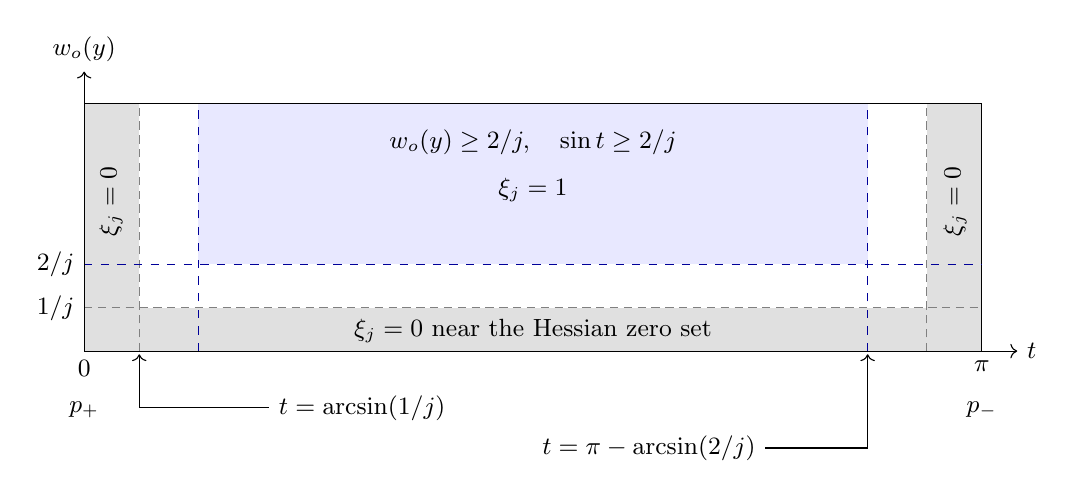
\begin{tikzpicture}[x=1cm,y=1cm,font=\small]
  \fill[gray!24] (0,0) rectangle (11.4,.55);
  \fill[gray!24] (0,.55) rectangle (.7,3.15);
  \fill[gray!24] (10.7,.55) rectangle (11.4,3.15);
  \fill[blue!9] (1.45,1.10) rectangle (9.95,3.15);
  \draw (0,0) rectangle (11.4,3.15);
  \draw[densely dashed,gray] (.7,0)--(.7,3.15);
  \draw[densely dashed,gray] (10.7,0)--(10.7,3.15);
  \draw[densely dashed,gray] (0,.55)--(11.4,.55);
  \draw[dashed,blue!60!black] (1.45,0)--(1.45,3.15);
  \draw[dashed,blue!60!black] (9.95,0)--(9.95,3.15);
  \draw[dashed,blue!60!black] (0,1.10)--(11.4,1.10);
  \node at (5.7,2.05) {$\xi_j=1$};
  \node[align=center] at (5.7,2.65)
    {$w_o(y)\ge 2/j,\quad \sin t\ge 2/j$};
  \node at (5.7,.26) {$\xi_j=0$ near the Hessian zero set};
  \node[rotate=90] at (.34,1.9) {$\xi_j=0$};
  \node[rotate=90] at (11.06,1.9) {$\xi_j=0$};
  \draw[->] (0,0)--(11.85,0) node[right] {$t$};
  \draw[->] (0,0)--(0,3.55) node[above] {$w_o(y)$};
  \node[below] at (0,0) {$0$};
  \node[below] at (11.4,0) {$\pi$};
  \node[left] at (0,.55) {$1/j$};
  \node[left] at (0,1.10) {$2/j$};
  \node[below,align=center] at (0,-.52) {$p_+$};
  \node[below,align=center] at (11.4,-.52) {$p_-$};
  \draw[<-] (.7,-.04)--(.7,-.72)--(2.35,-.72)
    node[right] {$t=\arcsin(1/j)$};
  \draw[<-] (9.95,-.04)--(9.95,-1.23)--(8.65,-1.23)
    node[left] {$t=\pi-\arcsin(2/j)$};
\end{tikzpicture}
\caption{The product cutoff on a suspended component.  The horizontal
variable is the suspension angle in
$\Phi(t,y)=(\sin t\,y,\cos t)$; the two end slices collapse to the
tips $p_+$ and $p_-$.  The vertical variable records the value of
$w_o(y)$, not a coordinate on $\Omega_o$.  Gray regions have
$\xi_j=0$, and the blue region has $\xi_j=1$; the intervening bands
contain the smooth transitions.  The scales are schematic, and no
shape or regularity of the Hessian zero set is represented.}
\label{fig:suspension-cutoff}
\end{figure}


On $\Omega_+=\{x\in\Omega:w(x)>0\}$, use the fields
\[
 h=w^a\sqrt{f(A,p,g)},\qquad
 Z_l=w^{2a}(G_{lijk}X_{ijk}+wM_l+P_l)
\]
constructed in Section~\ref{sec:flux}.  By Lemma~\ref{flux:field-bounds},
there is a fixed $C_F\geq1$ such that
\begin{equation}\label{cut:field-estimates}
 |h|\leq C_Fw^a,\qquad
 |\nabla h|\leq C_Fw^a(1+w+|X|),\qquad
 |Z|\leq C_Fw^{2a}(1+w+|X|).
\end{equation}
The constant depends only on $a$, the dimension $5$, the finitely many
coefficients defining $f,G,M,P$, and the positive lower bound
$f\geq\epsilon_*$.  In particular $C_F$ is independent of the cone,
$w$, $X$, and $j$.

For each fixed $j$, define $v_j=\xi_jh$ and $F_j=\xi_j^2Z$ on $\Omega_+$,
and extend them by zero where $w=0$.  These are smooth on the regular
closure of $\Omega$ and are supported away from the tips when present.
The same neighborhood argument as for $\alpha_j$ proves smoothness of
these extensions; it does not require $h$ or $Z$ themselves to extend
smoothly across $w=0$.  All products below containing one of these cutoff
factors or its derivative are likewise understood to be zero on $w=0$.
The mass $w^{2a}$, whose exponent is positive, has its ordinary value zero
there and involves no normalized tensor.

\begin{lemma}[Integrated comparison]\label{cut:integrated-comparison}
For each fixed $j\geq3$,
\begin{equation}\label{cut:three-errors}
 \epsilon_*\int_\Omega\xi_j^2w^{2a}\,dV
 \leq\int_\Omega\left(
    h^2|\nabla\xi_j|^2
   +2\xi_jh\langle\nabla h,\nabla\xi_j\rangle
   -2\xi_j\langle Z,\nabla\xi_j\rangle\right)\,dV.
\end{equation}
\end{lemma}

\begin{proof}
The interior comparison of Proposition~\ref{flux:interior-comparison}
gives
\[
 \int_\Omega\xi_j^2
       (4h^2+|\nabla h|^2+\epsilon_*w^{2a})\,dV
 \leq\int_\Omega\xi_j^2\diver Z\,dV.
\]
Apply the divergence theorem to the smooth field $F_j$.  In the
suspension one may first truncate the domain inside the two neighborhoods
where $F_j$ vanishes; the artificial end boundaries have zero flux.
On the regular side boundary the outward normal is $-N$.  Thus the
boundary comparison of Proposition~\ref{flux:boundary-comparison},
$N\cdot Z+Hh^2\geq0$, gives
\begin{align*}
 \int_\Omega\xi_j^2\diver Z\,dV
 &=-\int_{\partial\Omega}\xi_j^2\langle N,Z\rangle\,d\sigma
       -2\int_\Omega\xi_j\langle Z,\nabla\xi_j\rangle\,dV\\
 &\leq\int_{\partial\Omega}H(\xi_jh)^2\,d\sigma
       -2\int_\Omega\xi_j\langle Z,\nabla\xi_j\rangle\,dV.
\end{align*}
Corollary~\ref{geo:spherical-stability} applies to $v_j$ and bounds the
boundary integral by
\[
 \int_\Omega\bigl(|\nabla(\xi_jh)|^2+4\xi_j^2h^2\bigr)\,dV.
\]
Expanding the square and canceling the common terms gives
\eqref{cut:three-errors}.
\end{proof}

Every cancellation above is made before removing the angular cutoff.
For fixed $j$ and radial index $k$, the tests $\zeta_k(r)v_j$ from
Corollary~\ref{geo:spherical-stability} have compact support on the
regular Euclidean cone.  First take the variation parameter
$\varepsilon$ to zero on this fixed support; then let $k\to\infty$
in Equation~\eqref{geo:hardy-limit} to obtain the constant $4$.
The smooth extension collar and the allowed variation size may depend
on $j$ and $k$.  We now take $j\to\infty$ only in
Equation~\eqref{cut:three-errors}, which contains the positive mass
and three cutoff errors.  The energy and boundary terms have already
canceled for each fixed $j$.

\subsection{Vanishing of all three errors}

On $\Omega_{o,+}$, differentiation of $\alpha_j$ and
$|\nabla w_o|\leq|B_o|$ give
\begin{equation}\label{cut:original-cutoff-gradient}
 |\nabla_o\alpha_j|
 \leq\kappa\frac{|B_o|}{w_o}.
\end{equation}
To see the constant, wherever $\vartheta'(jw_o)\ne0$ one has
$1<jw_o<2$, so $j\leq2/w_o$; outside this transition region the derivative
is zero.  The same argument gives
\begin{equation}\label{cut:tip-cutoff-gradient}
 |\beta_j'(t)|\leq\frac{\kappa}{\sin t}.
\end{equation}
At every fixed point of $\Omega_{o,+}$, $\alpha_j=1$ and
$\nabla_o\alpha_j=0$ for all sufficiently large $j$.  At every fixed
$t\in(0,\pi)$ the corresponding statements hold for $\beta_j$.

Write $b_o=|B_o|/w_o$ on $\Omega_{o,+}$.  Let $E_{1,j}$, $E_{2,j}$,
and $E_{3,j}$ denote, in order, the three signed integrands on the right
of \eqref{cut:three-errors}.

First suppose $m_o=5$, so $\Omega=\Omega_o$, and set $K_n=1+M_o$.
Since $X=B_o/w_o$,
\[
 1+w+|X|\leq K_n(1+b_o),\qquad
 |\nabla\xi_j|\leq\kappa(1+b_o).
\]
Equations~\eqref{cut:field-estimates} and the preceding bounds give
\begin{equation}\label{cut:nonsuspended-domination}
 |E_{1,j}|+|E_{2,j}|+|E_{3,j}|
 \leq C_F^2(\kappa^2+4K_n\kappa)D_o.
\end{equation}
Indeed the three coefficient bounds are respectively
$C_F^2\kappa^2$, $2C_F^2K_n\kappa$, and $2C_FK_n\kappa$,
and $C_F\geq1$.  The dominator is integrable by
Lemma~\ref{cut:weighted-bochner}.  Each error is eventually zero at
every point of $\Omega_{o,+}$, and is defined to be zero on
$\mathcal Z_o$.  Dominated convergence therefore makes the right side
of \eqref{cut:three-errors} tend to zero.

Now suppose $m_o=4$.  Write $s_t=\sin t$ and use the suspension
coordinates $(t,y)\in(0,\pi)\times\Omega_o$.  The exact formulas in
Proposition~\ref{geo:suspension-data} give
\begin{equation}\label{cut:suspension-scaling}
 w(t,y)=\frac{w_o(y)}{s_t},\qquad
 |B(t,y)|^2
  =\frac{|B_o(y)|^2+3\cos^2(t)w_o(y)^2}{s_t^4},\qquad
 dV=s_t^4\,dt\,dV_o.
\end{equation}
In particular $\Omega_+=(0,\pi)\times\Omega_{o,+}$, and there
\[
 |X|=\frac{\sqrt{b_o^2+3\cos^2t}}{s_t}
       \leq\frac{\sqrt3}{s_t}(1+b_o).
\]
The warped metric gives the exact cutoff identity
\[
 |\nabla\xi_j|^2
 =\alpha_j^2|\beta_j'|^2
   +s_t^{-2}\beta_j^2|\nabla_o\alpha_j|^2,
\]
so \eqref{cut:original-cutoff-gradient}--\eqref{cut:tip-cutoff-gradient}
imply
\begin{equation}\label{cut:suspended-gradient-bounds}
 |\nabla\xi_j|\leq\frac{\kappa}{s_t}(1+b_o),\qquad
 1+w+|X|\leq\frac{K_s}{s_t}(1+b_o),\qquad
 K_s=1+M_o+\sqrt3.
\end{equation}
Multiplying the bounds for the three errors by the volume factor in
\eqref{cut:suspension-scaling} now gives
\begin{equation}\label{cut:suspended-domination}
 s_t^4\bigl(|E_{1,j}|+|E_{2,j}|+|E_{3,j}|\bigr)
 \leq C_F^2(\kappa^2+4K_s\kappa)
          s_t^{2-2a}D_o(y).
\end{equation}
This inequality is initially read on $\Omega_{o,+}$, and both sides are
assigned zero on $\mathcal Z_o$.  Its constant depends only on the
fixed certificate, $a$, $\vartheta$, and $M_o$, and is independent of
$j$, $t$, and $y$.  It also shows explicitly why the original weighted
$|B_o|^2$ estimate suffices: by \eqref{cut:original-dominator},
\[
 s_t^{2-2a}D_o(y)
 \leq 2s_t^{21/25}
       \bigl(w_o^{29/25}+w_o^{-21/25}|B_o|^2\bigr)
 \quad\hbox{on }\Omega_{o,+}.
\]
The right side is integrable with respect to $dt\,dV_o$, because
$21/25>-1$ and \eqref{cut:weighted-integrability} holds.  Every error
is eventually zero at each fixed $(t,y)\in(0,\pi)\times\Omega_{o,+}$.
Dominated convergence applied to \eqref{cut:suspended-domination}
therefore makes the right side of \eqref{cut:three-errors} tend to zero
also in the suspension.

\begin{theorem}\label{cut:exclusion}
The first dimension admitting a nonflat one-homogeneous global minimizer
cannot be $5$ or $6$.
\end{theorem}

\begin{proof}
If the first dimension were $5$ or $6$, the reductions would provide
exactly one of the two working domains just considered.  In either case,
the right side of \eqref{cut:three-errors} tends to zero.  On the original
component, however,
\[
 0<I_o:=\int_{\Omega_o}w_o^{2a}\,dV_o<\infty.
\]
Finiteness follows from boundedness and compactness.  Positivity follows
from $T_o\not\equiv0$ and continuity, which give an open subset of
$\Omega_o$ on which $w_o>0$.  In the nonsuspended case dominated
convergence gives
\[
 \lim_{j\to\infty}\int_\Omega\xi_j^2w^{2a}\,dV=I_o.
\]
In the suspended case \eqref{cut:suspension-scaling} gives instead
\[
 \lim_{j\to\infty}\int_\Omega\xi_j^2w^{2a}\,dV
 = I_o\int_0^\pi(\sin t)^{4-2a}\,dt
 = I_o\int_0^\pi(\sin t)^{71/25}\,dt>0.
\]
Here the dominating mass density is the integrable, everywhere defined
function $(\sin t)^{71/25}w_o^{29/25}$; its value is zero wherever
$w_o=0$.  These strictly positive limits contradict
\eqref{cut:three-errors}, since $\epsilon_*>0$.
\end{proof}

The known lower-dimensional classification gives $d_*\geq5$, and the
dimension-seven globally minimizing example gives $d_*\leq7$, as stated
in Section~\ref{sec:introduction}.  Theorem~\ref{cut:exclusion} excludes the only two
remaining possibilities below $7$.  Hence $d_*=7$, completing the proof
of Theorem~\ref{thm:main}.

\section{Regularity and sharpness of the dimension bound}
\label{sec:consequences}

We now pass from the classification of homogeneous global minimizers to
local free boundaries. This step uses the dimension-reduction theorem of
Weiss \cite{Weiss1999}, in the formulation
\cite[Theorem~1.4 and Proposition~10.13]{Velichkov2023}.

\begin{proof}[Proof of Corollary~\ref{cor:singular-set}]
Apply the cited dimension-reduction theorem with volume coefficient one
on balls compactly contained in $D$. Its inputs are uniform flatness
regularity, linear nondegeneracy, compactness of blowups, and the fact that
all blowup limits are homogeneous global minimizers. These are the
constant-coefficient results used in Proposition~\ref{red:regularity};
flatness regularity is \cite[Theorem~8.1]{Velichkov2023}.
The theorem gives an empty singular set below $d_*$, local finiteness in
dimension $d_*$, and Hausdorff dimension at most $n-d_*$ above it.
Theorem~\ref{thm:main} sets $d_*=7$. Smoothness at each regular point
follows from Proposition~\ref{red:regularity}(iii). A countable cover by
interior balls gives the assertions on $D$.

For sharpness, let $U$ be the nonflat global minimizer in $\R^7$ of
De Silva and Jerison \cite[Theorem~1.1]{DeSilvaJerison2009}, and set
$U_n(x,y)=U(x)$ on $\R^7\times\R^{n-7}$.
Repeated application of Proposition~\ref{red:suspension} shows that $U_n$
is globally minimizing. At each point $(0,y_0)$, every rescaling of $U_n$
is $U_n$ itself, by homogeneity and translation invariance in $y$.
It cannot be flat: a half-space normal would have zero $y$-component,
forcing $U$ to be flat. Thus
$\{0\}\times\R^{n-7}\subset\operatorname{Sing}(U_n)$.
Its dimension is $n-7$, and the proved upper bound gives equality.
\end{proof}


\appendix
\section{Complete coefficient tables}\label{app:tables}

The following two tables specify the polynomials used in
Section~\ref{cert:table-I} and the comparison forms in
Section~\ref{cert:gram}. Every coefficient printed below is an integer
numerator with denominator
\[
Q=250000.
\]
Leading zeroes in monomial codes are significant. All rows and all block
headers are included.

\subsection{Decoding and block conventions}\label{app:decoding}
For nonnegative rank, read a monomial code in consecutive triples.
Its first triple $h\,b\,j$ contributes
$g^h(\tr A^3)^b w^{[j=1]}z^{[j=2]}$.
Each subsequent triple $u\,v\,k$ is an unoriented edge carrying $A^k$,
with $A^0=\Id$. Endpoints $0,\ldots,r-1$ denote the free slots in order,
$5$ denotes a copy of $p$, and $6$ a copy of $\ell$;
three occurrences of $7$ are contracted with one $X$,
and three occurrences of $8$ with a second copy.
Multiply all factors and contract all nonfree slots.
There are no additional multiplicity factors; see
Section~\ref{cert:decode}.

In Table~I the first field specifies the polynomial, the second its monomial,
and the third its coefficient numerator. The free-slot orders are
$U_{jk}$, $K_{lijk}$, $M_l$, and $P_l$, while $f$ has rank zero.
The numbers of rows for $(f,U,M,P,K)$ are $(34,57,74,32,34)$,
for a total of $231$.

Each line of Table~II beginning with \texttt{@} starts a separate block
and gives its rank, projection label, and multiplier mode.
For each coefficient column, sum the monomials with the coefficients
in that column divided by $Q$ to obtain a tensor $J_c$.
For nonnegative rank the block contributes
$\rho\sum_c\langle J_c,\Pi J_c\rangle$ to $\Gamma$,
where the modes \texttt{I} and \texttt{B} mean
$\rho=1$ and $\rho=\chi=1-|p|^2-g^2$, respectively.
The labels \texttt{none}, \texttt{anti}, \texttt{sym}, and \texttt{hook}
specify exactly the operators of Section~\ref{cert:projections};
they do not instruct any further normalization of the coefficients.
Identical headers in different positions still define distinct blocks.

For rank $-1$, the four code digits instead give the four individual
exponents of $x_1,x_2,x_3,x_4$. The block contributes to $\Lambda$
the average over all $24$ permutations of
$\rho\sum_c J_c^2$.
Here \texttt{I} means $\rho=1$, while \texttt{H} means
$\rho=\sum_i x_i=-\lambda$.
The averaging and boundary normalization
$R=\sum_i x_i^2+(\sum_i x_i)^2=1$ are those of
Section~\ref{cert:gram}.
Table~II contains $21$ blocks: $19$ interior blocks with $529$ rows and
two boundary blocks with $14$ rows each, hence $557$ coefficient rows
in total. Each block retains its own number of coefficient columns.

\subsection{Table I: the multiplier coefficients}\label{app:table-I}
The columns below read from top to bottom, first on the left and then
on the right.
\begin{multicols}{2}
\begin{Verbatim}[fontsize=\footnotesize]
f 000 172575762
f 200 -265322011
f 400 301491831
f 600 -44526835
f 800 14565793
f 000550 -54772531
f 200550 219932290
f 400550 52506144
f 600550 9630205
f 000550550 137906751
f 200550550 106469818
f 000550550550 -131450161
f 200550550550 46298458
f 000550550550550 19137894
f 000551 119093719
f 200551 -79672895
f 400551 -9715716
f 000550551 -60378744
f 200550551 14546676
f 400550551 -57731025
f 000550550551 156426055
f 200550550551 -335208469
f 000550550550551 -114479609
f 000552 36551855
f 200552 -61391750
f 400552 -54261369
f 000550552 47470176
f 000551551 38322040
f 200550552 -123645111
f 200551551 21745017
f 000550550552 -27358875
f 000550551551 -10633583
f 000551552 -63061863
f 200551552 -7335033
U 000500510 209038273
U 200500510 -16767570
U 400500510 -283063959
U 600500510 -30248846
U 000550500510 -136083135
U 200550500510 -427782476
U 400550500510 -31623665
U 000550550500510 10893857
U 200550550500510 546331605
U 000550550550500510 427088076
U 000011 170760340
U 200011 -1206356
U 400011 121148296
U 600011 41094485
U 000550011 159740708
U 000500511 -12972332
U 200550011 -371328968
U 200500511 158604412
U 400550011 323446445
U 400500511 -150167309
U 600550011 -71599174
U 000550550011 -98427304
U 000550500511 -66406904
U 000551500510 161528440
U 200550550011 360663252
U 200550500511 -17938869
U 200551500510 84273648
U 400550550011 -202347674
U 400550500511 -24865978
U 400551500510 20187308
U 000550550550011 -95478557
U 000550550500511 243609372
U 000550551500510 -260094552
U 200550550550011 -175753712
U 200550550500511 -115703729
U 200550551500510 -18269297
U 000550550550550011 52505668
U 000550550550500511 -136286395
U 000550550551500510 124924734
U 000551011 -34002037
U 200551011 -87426923
U 400551011 -16110396
U 000550551011 -51017991
U 000551500511 182661478
U 000552500510 -212756173
U 200550551011 98857514
U 200551500511 -82275068
U 200552500510 -68411390
U 000550550551011 -365742
U 000550551500511 121156685
U 000550552500510 65143542
U 000551551500510 -118149741
U 000551551011 20474336
U 000552500511 13163650
U 200551551011 19565853
U 200552500511 -13163652
U 000550552500511 -13163652
M 000500 119808440
M 200500 -78615281
M 400500 58172228
M 600500 117063991
M 000550500 -8257673
M 200550500 -246670620
M 400550500 546437417
M 000550550500 -304458502
M 200550550500 147099465
M 000550550550500 -259741510
M 000501 13135177
M 200501 230900882
M 400501 503642015
M 600501 113276750
M 000550501 284895091
M 000551500 -41618173
M 200550501 895262372
M 200551500 -64307015
M 400550501 -501973998
M 400551500 203881659
M 000550550501 -251554675
M 000550551500 -68782868
M 200550550501 -641088126
M 200550551500 179691016
M 000550550550501 139784474
M 000550550551500 -40969083
M 000502 -24304787
M 200502 -622936552
M 400502 268923235
M 600502 168388434
M 000550502 -108635150
M 000551501 318683040
M 000552500 33990338
M 200550502 361921940
M 200551501 153090065
M 200552500 -747048669
M 400550502 558178192
M 400551501 -1665598002
M 400552500 1296406233
M 000550550502 411493367
M 000550551501 -121808407
M 000550552500 11773023
M 000551551500 67252403
M 200550550502 -446325581
M 200550551501 79505560
M 200550552500 125885807
M 200551551500 -19251826
M 000550550550502 -408356086
M 000550550551501 2958960216
M 000550550552500 -2765855048
M 000550551551500 -39050858
M 000503 31451284
M 010500 -111968845
M 200503 461057708
M 210500 221824980
M 400503 -412407021
M 410500 -101679590
M 000550503 121978129
M 000551502 -465236572
M 000552501 -85409256
M 000553500 501586157
M 010550500 189809541
M 200550503 -457984830
M 200551502 -131436746
M 200552501 1156439419
M 200553500 -438673045
M 210550500 -199478216
M 000550550503 -37100467
M 000550551502 376993983
M 000550552501 216559416
M 000550553500 -236527028
M 000551551501 118549720
M 000551552500 -289837183
M 010550550500 -92636597
P 100500 311718636
P 300500 -206555629
P 500500 -10345809
P 700500 69636002
P 100550500 -335187565
P 300550500 141480631
P 100550550500 -48726916
P 300550550500 -59898908
P 100550550550500 -130179927
P 700501 664922213
P 100551500 37613817
P 500550501 2068537473
P 100550551500 -80492409
P 300550550501 -3956993330
P 300550551500 2941040012
P 100550550550501 -4535791726
P 100550550551500 2719912082
P 100552500 59422497
P 300552500 -112216670
P 100550552500 160359392
P 100551551500 -210782200
P 100551502 -955698012
P 100552501 289629865
P 100553500 289477038
P 300551502 290419431
P 300552501 -244526547
P 300553500 -89919120
P 100550551502 372091130
P 100550552501 -196017256
P 100550553500 -130830861
P 100551551501 223993677
P 100551552500 -287868455
K 000500520131 -395492688
K 200500520131 557130979
K 400500520131 -208630461
K 000550500520131 265035499
K 000500511520530 177271543
K 200550500520131 -288587200
K 200500511520530 -18030270
K 000550550500520131 -29990138
K 000550500511520530 -153812921
K 000500511231 142329663
K 200500511231 -265174093
K 400500511231 209730769
K 000550500511231 -47161546
K 000551500520131 126782841
K 000500512520530 -310431451
K 200550500511231 134860957
K 200551500520131 -72013133
K 200500512520530 90786861
K 000550550500511231 -155714998
K 000550551500520131 4534988
K 000550500512520530 171186722
K 000551500511520530 -64357492
K 000500512231 380733573
K 200500512231 -425302994
K 400500512231 164988206
K 000550500512231 -325733710
K 000551500511231 -84676007
K 000552500520131 6581825
K 200550500512231 449829666
K 200551500511231 7194909
K 200552500520131 -6581826
K 000550550500512231 153898314
K 000550551500511231 46595618
K 000550552500520131 -6581826
\end{Verbatim}
\end{multicols}

\subsection{Table II: the comparison coefficients}\label{app:table-II}
\noindent The block headers are part of the data.
\begingroup\clubpenalty=10000\widowpenalty=10000
\begin{Verbatim}[fontsize=\footnotesize]
@ 0 none I
001 12
\end{Verbatim}
\begin{Verbatim}[fontsize=\footnotesize]
@ 0 none I
002 184
\end{Verbatim}
\begin{Verbatim}[fontsize=\footnotesize]
@ 1 none I
000771700 -638806
000750750701 -983284
000750751700 1320922
000750750750501 805293
000750750701550 1754296
000600 503057
000600551 -1946630
000600550551 1923242
000651501 -2068563
000601551 -1021342
001502 -3593596
001550502 4994642
\end{Verbatim}
\begin{Verbatim}[fontsize=\footnotesize]
@ 1 none B
000602 1754266
000601551 -1522955
000602550 -2522248
\end{Verbatim}
\begin{Verbatim}[fontsize=\footnotesize]
@ 2 sym I
000750700710 1391786 1177679
200750700710 -635584 -1188129
000750750700510 -669474 -759226
200771700510 145856 439798
000771750500510 -365548 1663410
000771700550510 333085 -1276634
000750750750011 898927 557074
000750750700511 -311872 -891024
000750750701510 -41287 -1733462
000750751700510 -93961 1393977
000750700710551 113136 227458
000771750011 57792 -1227345
000771700511 -2146827 33344
000771701510 -214285 799004
200771750011 1112073 309389
200771700511 1556631 843960
200771701510 -294789 -594312
000771750550011 -13597 795429
000771750500511 -329731 1039673
000771751500510 -836011 1028480
000771700550511 216212 -603835
000771700551510 1434254 -827393
000771701550510 656139 -279125
000600510 -388425 -131346
000600550510 -477571 -239908
000650011 1059131 288654
000601510 252356 -522796
200650011 -1055033 202800
200601510 422375 425949
000650550011 -1586221 -893296
000650500511 393362 557037
000651500510 573436 -1067580
000600550511 -290759 380780
000600551510 -876849 -172942
000651011 16748 -630547
000601511 18986 878826
000602510 -32503 767092
200651011 -572999 -197116
200602510 -62643 182099
000651500511 -99714 99762
000652500510 1165974 -802821
000601551510 -1273792 -46716
000602550510 151518 380083
001500510 -818099 -26218
201500510 551865 2425759
201011 807336 716540
401011 -1809265 -594
001550011 1952714 -432372
001500511 -970041 4080275
201550011 -3494733 -1591876
201500511 -2942057 1178858
001550550011 -2197984 152320
001550500511 -1126597 -3610821
001551500510 1302795 2046516
201012 453912 -635196
001550012 802719 479394
001500512 1149385 1541894
001501511 -570358 863506
102550011 2753121 -35533
102551011 -7449352 0
102500512 712433 -1155568
102501511 -648523 1532248
\end{Verbatim}
\begin{Verbatim}[fontsize=\footnotesize]
@ 2 anti I
000750750700510 -971778 -593070 595799
000750750700511 1851218 390321 -1032828
000750751700510 -2221492 -384831 773149
000771700511 1671121 1696523 -468940
000771701510 1285532 -64095 -352045
200771700511 362947 -2582045 -2929678
200771701510 -181856 1690707 -1313034
000771750500511 977807 -1459534 1360532
000771700550511 -1653489 -1171267 -3601252
000771700551510 1692989 13676 305417
000600511 912880 512840 1024400
000600550511 1022451 2751390 2442625
000601511 2261978 -1322826 -210765
000602510 2192414 -515944 -180511
000651500511 2409290 -1068889 -1803516
000601550511 -1177522 2817530 -34700
000601551510 1957710 -3140417 -720539
000602550510 -261398 1630593 -956020
001500512 -130602 5301163 0
102500512 -5486646 0 0
\end{Verbatim}
\begin{Verbatim}[fontsize=\footnotesize]
@ 2 sym I
100750700710 386912 590109 2476735 909989
300750700710 -324620 -1836020 1070522 -709211
100750750700510 207036 867875 -1315712 -1562386
100750700710550 -2292260 -2320517 -877238 -137767
100771700510 679665 129424 -1701690 711883
300771700510 -691965 -2367998 -600979 1614358
100771700550510 71429 -500416 812821 -488846
100750750750011 425332 -329290 685878 -37805
100750750700511 1670160 798393 1099878 1675685
100750750701510 618399 661946 -1024107 -525490
100750751700510 82393 -436965 -872804 890466
100750700710551 -1425953 113042 -858760 -800516
100771750011 625914 918398 -1118557 -279579
100771700511 631990 1190528 -803355 693822
100600510 747288 856865 765295 19368
300600510 -196289 641398 -318973 -1435522
100600550510 -2242557 1145358 1750835 25513
300600511 -350390 -359430 -160354 -354520
300601510 -998743 -242982 -243886 303678
100650500511 1317416 -1625911 1342770 527410
100651500510 620553 -221636 -278822 -584012
100600550511 -563526 294802 -1407035 -675807
100601550510 -1165326 -290961 158430 23084
100651011 -1073379 74678 -692146 131418
100601511 610649 -693839 -174161 54662
100602510 1468661 -1066444 257457 -1866082
101011 891879 -816951 -355999 -242185
301011 -128043 -1656108 -3338499 0
101550011 262135 -1773969 -1081346 1502914
101012 247618 992865 441378 -984847
301012 273293 -835560 84484 79079
101550012 -968245 -1440718 -66260 1176036
101551011 -540581 4211626 0 0
101500512 571373 -2763887 -288603 -351329
101501511 -633764 1126754 22804 -757142
002500510 2095639 323489 -1897011 484510
002550500510 -2013271 -345687 1721490 -160235
002011 -22315 614400 440061 106088
202011 -789708 -1586444 435018 1192156
402011 176801 1776607 -935958 110464
002550011 -752649 2387292 158922 -11589
002500511 965395 122624 -1704548 -1591006
202550011 713344 -2161421 1573837 -1092257
202500511 4263736 0 0 0
002550550011 651775 -2930070 -692641 103706
002550500511 -241365 -1063259 672383 277457
002551500510 -1497924 882585 1136032 805365
002551011 14258 -733558 -562699 359850
002500512 -1418407 941987 1726713 -1244268
002501511 598151 -558439 -599397 139693
\end{Verbatim}
\begin{Verbatim}[fontsize=\footnotesize]
@ 2 anti I
300771700510 -4701036 0
100750750701510 -1924807 -3971273
\end{Verbatim}
\begin{Verbatim}[fontsize=\footnotesize]
@ 2 sym B
000750700710 1123954 88221 -1701307 30701 738750
200750700710 270992 1585448 -437804 -115089 -193670
000750750700510 1172241 -871881 1057083 321028 -649097
000750700710550 -524706 1366647 827758 -1278231 500667
000771700510 864484 287922 -68675 62361 -539022
200771700510 775795 2191982 950393 914569 -166597
000771700550510 277543 -125661 661263 -1877406 74958
000750750750011 -334486 169170 -871041 -791399 -94389
000750750700511 -975320 58917 -494669 -25254 -1254928
000750750701510 -1503410 -485996 1281582 -196803 63872
000750751700510 -184521 435306 51628 1182804 106124
000750700710551 852497 -216529 665736 60101 1484575
000771750011 169826 196263 532547 536554 -474267
000771700511 -1010968 -842722 1104099 -283384 -997589
000771701510 652964 -776198 -18629 -4645 767925
000600510 -785042 -1594270 -1342680 -873445 1197286
200600510 -1131334 -822268 -1011918 773265 -1414931
000600550510 -1127966 720812 -94366 3116158 0
000650011 -912533 515978 700674 -905482 -690654
000600511 -885433 -542182 377374 1618276 949245
000601510 -75331 228090 -522865 124191 -472481
200601510 225414 309487 730722 372893 -484343
000650550011 632175 386796 -1057545 494534 31994
000650500511 -135981 -192395 -255297 -1158355 -1164507
000600550511 -755722 -515530 -883058 -395726 -81284
000600551510 219256 808172 -566082 901822 1273544
000651011 825451 -630349 -288434 160119 -296916
000602510 -202711 542117 386813 746612 -1023986
001500510 -772925 -854066 -27932 -390900 -243719
001011 -224989 -518216 209663 226840 265618
201011 410735 -748292 -1336059 -978726 -1844315
001550011 777323 1939452 -296868 137265 -763612
001500511 1785297 -3689052 0 0 0
001012 504959 -153386 -533263 -398633 -253956
201012 33011 404249 365930 -462942 -522985
001550012 -422915 928502 262771 13083 730837
001551011 474507 -1487386 -270414 650144 346202
001500512 3326366 -1640992 -12535 829591 -679038
001501511 -1859882 817429 -223272 -262739 -290165
102500510 -478971 -135787 -3191296 0 0
102011 256382 1937630 -477578 -3953 68002
302011 -893937 -2987523 1695406 937674 871113
102550011 282559 3032355 303938 -524882 -396049
102500511 -5673921 0 0 0 0
\end{Verbatim}
\begin{Verbatim}[fontsize=\footnotesize]
@ 2 anti B
000771700510 -470106 -1867823
200771700510 -1539213 -3753948
000771700550510 2293133 3344366
000750750700511 -1181347 3094806
000750750701510 -1994876 -336384
000750751700510 -654677 -388774
000771700511 4870801 -1507979
000600510 -786617 -2630683
000600550511 -1157549 1248692
001500511 7658597 984973
001500512 9501737 0
\end{Verbatim}
\begin{Verbatim}[fontsize=\footnotesize]
@ 2 sym B
100750700710 -430860 3401943
100771700510 2216725 -501573
100771750011 -324461 488844
100771700511 -460201 -3052123
100602510 -29622 190280
101500510 -345767 -2635854
101011 1458366 -2486198
301011 1803625 142753
101550011 3135810 519582
101500511 4871812 0
101012 -1600522 2717619
002500510 2853790 -389130
002011 -1177206 1455424
202011 2486645 -2061003
002500512 226083 1738130
\end{Verbatim}
\begin{Verbatim}[fontsize=\footnotesize]
@ 3 sym I
000700710720 -113771 255769 111215 -454364
200700710720 -612356 -336756 260567 -434709
400700710720 187848 12317 315606 237812
000750700710520 900121 -709342 -2099958 0
000700710720550 -430894 -181858 563914 -156096
200750700710520 437857 -822749 -59817 -296875
200700710720550 707274 -39518 300182 393708
000750750700510520 -571399 -327143 1016828 -283559
000750700710550520 217996 733662 -203570 -157699
000700710720550550 -129019 -36697 138224 524819
000771700510520 586900 -74005 -121132 -122868
000750750700121 -462420 -167189 10152 -995469
000700710720551 324263 -97555 -31078 79005
200771700510520 -1704404 645318 -797565 -366568
200750750700121 -653595 -82465 495776 672582
000771750500510520 99472 9389 758 -75480
000771700550510520 -982221 -270970 126195 249382
000750750750500121 -196787 2174 -150592 189900
000750750700550121 398559 73300 -15538 1100718
000750750700510521 1017001 85910 -85403 -114698
000750750701510520 -2470 224111 433730 114651
000750751700510520 21519 194168 -176031 -444752
000750700710551520 -1114090 429871 237715 -60368
000771700121 304609 294448 -331206 192661
200771700121 -60418 370467 -581683 931857
000771750500121 -415651 -57300 1135378 -577
000771700550121 701709 -266536 -544044 -372
000771700510521 -659682 506640 659123 405954
000771701510520 265617 -292435 -404728 -100735
000750750701121 18224 139410 -137979 40692
000750751700121 -36447 -278820 275957 -81384
000600510520 -899921 -1075432 -358643 733633
200600510520 385602 459559 532440 -174373
000600550510520 1350470 1101595 130507 -650217
000600121 -112918 -833408 3283 336677
200600121 -280772 593983 255592 -62606
400600121 199724 -44666 -281861 7161
000650500121 574659 520651 586199 499213
000600550121 -635944 683654 -461102 -386753
000600510521 151416 109514 1182094 -86343
000601510520 -335272 216945 -2525 -226735
200650500121 -358009 323248 71453 -757989
200600550121 725371 -296915 -476424 82812
200600510521 376728 14961 -64841 327020
200601510520 144429 294432 -112571 364619
000650550500121 -571391 -817993 -883836 -283605
000650500510521 368142 287873 71877 531508
000651500510520 245134 -554713 -13119 -134830
000600550550121 360296 129561 131379 -204106
000600550510521 220585 -55552 -310575 123432
000601550510520 81688 178086 -318606 114806
000601121 -43340 115549 -299646 274416
200601121 351342 -257317 287701 -80004
000651500121 -265 -306814 47933 -190062
000600551121 24164 -60022 9704 -502077
000601550121 22042 -133331 497455 -284993
000601510521 54994 -97006 -456467 154307
000602510520 316820 377069 385482 2722
001500510520 175400 -610502 262613 498453
001500121 270953 1089209 -894330 -1087117
201500121 -2817754 0 0 0
001550500121 -64359 -995858 1321040 876172
001500510521 818582 -1242137 -464133 -352
001500122 -290488 -749992 533305 -216922
001501121 228018 121871 -1438294 -159411
201500122 581286 391875 -432476 -82568
201501121 759430 457624 -1528682 -569408
001550500122 -194952 787664 -496482 -263483
001550501121 -100036 -315655 212934 -135339
001551500121 4781 339166 1701093 191517
001500510522 438901 -206515 -1697183 -497546
001500511521 837267 366075 591534 -903944
102500510520 -2096422 -555979 -1063939 -332549
102500121 -1196882 -774162 229623 -968007
302500121 -158570 2534250 0 0
102550500121 1589062 64468 561859 -547323
102500510521 1459032 761992 -18106 1397641
102501121 -92705 -956776 286224 1637465
\end{Verbatim}
\begin{Verbatim}[fontsize=\footnotesize]
@ 3 hook I
000750700710520 -521222 561024 -561794 1052779 -495550
200750700710520 71379 -1012982 644900 5650 501292
000750750700510520 402987 -219447 -626761 -216393 402848
000750700710550520 -8001 -496420 547496 92579 -59265
000771700510520 -142929 713981 -67315 234399 244214
000750750700121 758990 -932613 -95069 -624172 652182
200771700510520 136872 -2833269 0 0 0
200750750700121 410563 890616 267929 843072 400842
000771700550510520 -94358 -1111623 117231 -178880 -873801
000750750750500121 -516610 372353 -315103 142027 -431781
000750750700550121 -487810 512416 199453 257643 709868
000750750700510521 -242753 38245 328922 390069 -260854
000750750700511520 -124564 146735 159175 478474 -401860
000750750701510520 103877 -149602 214675 -654790 321761
000750751700510520 -66938 -586167 -705386 -193823 207964
000750700710551520 -214009 -58852 -175575 503511 293821
000771700121 -714002 830419 -553629 -218156 -632060
200771700121 -1695971 -1249692 262718 -163683 295847
000771750500121 459356 -462844 600575 1873546 -501623
000771700550121 -894867 258654 93799 -489902 337300
000771700510521 -177274 -531780 212834 428441 569484
000771700511520 659247 -665793 446749 -348691 241301
000771701510520 -512759 -75335 -171988 709731 -5471
000750750701121 -175171 -106960 49079 -186227 -41325
000750751700121 350342 213920 -98158 372454 82649
000600510520 781928 -857622 -775483 1574702 495170
200600510520 -436371 772702 420563 -1389626 158574
000600550510520 -188177 1185337 422173 -697494 89039
000600121 -174456 -452110 1107721 719114 -339614
200600121 575087 477162 -1219698 -299117 543378
400600121 -323376 -218129 -102949 -54388 -553854
000650500121 27383 -107674 -702286 -330723 1709805
000600550121 1104948 752674 -1314904 -273205 -486768
000600510521 -191372 453079 1148360 -743039 213125
000600511520 -945043 86766 288577 -1327960 1483607
000601510520 88069 -67576 359002 123744 828607
200650500121 -1072923 443728 -868707 -247959 -719466
200600550121 -1416409 -1139165 878506 -381550 -1041027
200600510521 484829 -407429 -1279351 344883 396416
200600511520 273822 -83689 -23771 541818 -93062
200601510520 1269710 -595989 -725521 -508102 -968063
000650550500121 -912102 -107501 354623 302791 -389373
000650500510521 146766 -71825 -397270 479290 -588396
000600550550121 35085 -683028 148446 -371512 68128
000600550510521 -42888 349274 -901813 393417 522038
000600550511520 136766 215868 -410901 655309 -328001
000600551510520 381546 -306483 -220658 713294 -376417
000601550510520 122129 380094 -201606 29113 -229702
000601121 -297793 -200797 -357156 151714 83189
200601121 379667 -316478 1894 27814 -100117
000651500121 274768 1623518 1095549 -298694 769624
000600551121 -61936 151106 -600337 -565738 -905939
000601550121 -382039 -589283 -353162 774352 132457
000601510521 583607 -307759 150598 -143259 -344160
000601511520 643712 730410 859370 -337692 -182581
000602510520 -75121 339094 691943 -1345435 197464
001500121 -1494181 503416 908836 279260 -884597
201500121 1193310 -1354927 -782187 -94653 -1775124
001550500121 888287 156494 -1067876 85686 -251732
001500510521 -220586 817779 837882 -345286 225358
001500122 536790 -391686 -101844 -512835 579492
001501121 -331317 -847838 404838 -187537 756081
201500122 109188 -545375 679601 -31854 -746597
201501121 -2043083 -257885 -1617158 -1356106 946843
001550500122 -145862 317672 46224 -302265 366894
001550501121 -355398 1797394 -848219 95142 -1825951
001500510522 451367 -459915 1561510 171732 -1052563
001500511521 1010744 1710544 667697 2008851 0
102500121 -2029395 1305940 -1413287 -46785 -1170911
302500121 67942 284188 2810795 0 0
102550500121 -3797108 0 0 0 0
102500510521 407122 508125 -1070203 -734001 129444
102501121 764808 -802563 -1980310 422533 -196982
\end{Verbatim}
\begin{Verbatim}[fontsize=\footnotesize]
@ 3 sym I
100700710720 763442 201492 207522
300700710720 95273 -398706 -285657
100750700710520 -178597 -610639 -380231
100700710720550 87253 171084 29880
100750750700121 677852 -480761 -297581
100700710720551 -131663 307969 -65446
100771700121 -722948 498495 -744992
300771700121 -20413 -264875 24427
100771750500121 -856424 52791 -576220
100771700550121 -311085 -77567 662311
100771700510521 -290923 -342609 163397
100771701510520 967581 380184 518451
100600121 -62632 -367368 -337983
300600121 -232214 131223 1210412
100650500121 535397 253023 618813
100600550121 -114157 -986522 366025
100601510520 -222496 -945885 -791072
100601121 487623 -284646 47079
100651500121 320106 -419828 145656
100600551121 -250772 7204 60159
100601550121 -521317 216628 121550
100601510521 70667 785595 -223676
100602510520 -288917 -47520 -555205
101500121 1657716 1252785 -819550
301500121 -1268874 -1299493 359066
101550500121 -1560884 -844675 481939
101500510521 -948453 -2295369 0
101501121 -1137151 373989 -1131226
202500121 2601109 0 0
002501121 1111694 -645730 556437
202501121 -793881 1173902 348366
002550501121 -1007658 503344 -581407
\end{Verbatim}
\begin{Verbatim}[fontsize=\footnotesize]
@ 3 hook I
100750700710520 825602 -647783 -380956 627925
100750750700121 -609729 889144 939275 -551336
100771700121 553682 -757497 47709 76332
300771700121 52101 1440744 -29071 462803
100771700550121 338103 740201 -1034686 632136
100771700510521 -868620 -616124 659662 261166
100771700511520 -1302505 642931 386513 -173661
100600121 407862 -1621952 12844 -258039
300600121 -312260 698088 1526313 39006
100650500121 -1642917 -1068956 -856878 621314
100600550121 846350 185586 1899285 0
100600510521 -452723 -233514 -353926 -552612
100600511520 -735715 -139231 -122756 -1159566
100601510520 -891337 -1099752 314149 874177
100601121 -263510 -128947 -308339 -577662
100600551121 30015 -282112 -262490 -46840
100601550121 -363384 -588474 -188664 -768767
100601511520 -104651 121394 -405086 518512
100602510520 270194 -545783 524591 488199
101550500121 2823724 701590 -1140106 119387
101500122 -2379602 158372 532980 -216690
101501121 3974290 0 0 0
002500121 2422490 -2159158 0 0
202500121 -1136051 1092498 316605 375255
002550500121 -2217477 2065768 28247 56618
002501121 1268851 -686257 -535256 -751379
202501121 745085 1046811 125241 528487
002550501121 995369 1322195 391113 529705
002551500121 -2047579 -591242 193597 116743
002500510522 -323862 385594 269999 -545727
002500511521 1649181 -126174 -960119 202680
\end{Verbatim}
\begin{Verbatim}[fontsize=\footnotesize]
@ 3 sym B
000700710720 846861 -24321
200700710720 -587033 -427093
000750700710520 -1965133 -378988
000700710720550 825913 52688
000750750700121 553913 -164685
000771700121 -881954 151526
200771700121 -146368 443742
000771750500121 196867 256600
000771700550121 -174415 371933
000771700510521 918983 174066
000771701510520 103141 -271115
000750750701121 30207 -350636
000750751700121 -60414 701272
000600121 -134478 -616847
200600121 310759 1224961
000600550121 -456564 -388139
000600510521 -546360 388670
000601510520 150147 32880
000651500121 423955 -143460
000601510521 -575200 -49553
001500121 852643 -356042
201500121 137609 930402
001550500121 -170265 1104176
001500510521 -1212241 -484563
001500122 1303787 -240027
102500121 470182 -1041354
102501121 -2194212 0
\end{Verbatim}
\begin{Verbatim}[fontsize=\footnotesize]
@ 3 hook B
000750700710520 176217 -621830 -368016 -355219
000750750700121 669944 32834 222054 469807
000750700710521 -120742 -15513 373406 -3228
000771700121 -478208 110067 -148363 195976
200771700121 -172500 -1260542 -116598 -977491
000771750500121 1150872 -528405 947239 -36745
000771700550121 -696098 -439222 -238840 519754
000771700510521 220554 -62361 1356486 -44941
000771700511520 519253 461994 1434358 -90787
000771701510520 158972 -272179 555240 782647
000750750701121 62126 429282 35836 -241432
000750751700121 -124251 -858565 -71672 482863
000600121 -466987 816933 -112888 482852
200600121 245653 -1911953 0 0
000650500121 502203 -461250 -572970 -1626003
000600550121 114763 177125 41031 -397565
000601121 -462310 137283 -146876 -357410
000651500121 557962 98581 -449567 -270660
000601550121 483182 198409 168823 502176
000601511520 236903 38024 -575403 43162
000602510520 -819836 -51597 -494829 -376153
001500121 -537725 648487 -1190924 372381
201500121 -158924 -560572 1216153 157041
001550500121 -776297 -447725 1755130 0
001500510521 514745 293834 1370684 -929697
001500122 271133 251595 709127 184032
001501121 756147 333820 -1452866 -93607
102500121 -3095117 0 0 0
102501121 -2016691 -876281 -216593 -1560114
\end{Verbatim}
\begin{Verbatim}[fontsize=\footnotesize]
@ 3 sym B
100700710720 489692 598090
300700710720 -395941 -186631
100750700710520 156230 -1702877
100700710720550 -1161498 117080
100771700510520 399918 670413
100750750700121 296147 758447
100771700121 -612228 -210536
100600510520 19208 -830671
100600121 578884 306756
100600510521 -378724 -222954
100601121 -379693 84297
101500121 2749187 0
101500122 -30164 -776315
101501121 -1310240 -1277716
002500510520 741853 689530
002500121 -840735 1782441
202500121 1035886 -672361
002550500121 -1490277 -1501412
002500510521 859145 -683392
002501121 -259132 1352466
\end{Verbatim}
\begin{Verbatim}[fontsize=\footnotesize]
@ 3 hook B
100750700710520 -130387 1549320
100771700510520 -325730 2482101
100750750700121 509197 -841014
100771700121 -1556447 1491379
100600121 90411 -1200728
300600121 348733 328763
100600550121 497934 1094517
100600510521 -324819 -165030
100600511520 808473 -127941
100601510520 671603 976248
101500121 1417347 -444112
101500122 1223107 1177793
101501121 -2891915 -774938
002500121 -3515717 0
202500121 2603006 -45060
002550500121 1454140 -2066553
002500510521 -221322 -2086794
002501121 -1023409 -1933433
\end{Verbatim}
\begin{Verbatim}[fontsize=\footnotesize]
@ -1 none I
1000 -7510150 892635 2182767 23202 -4016
0100 -5873297 -966404 1065127 891160 -4153
0010 -7594462 3164488 32982 23257 -4265
0001 -6664095 -676125 -2074840 -90371 -141368
2000 10527925 -1288669 -3350633 0 0
1100 13562510 -782596 -3072444 -1185008 -525859
1010 14954300 -3513649 -2045232 175643 711822
1001 16001742 0 0 0 0
0200 7976754 1609001 -1608780 -1353027 0
0110 15395603 -1696042 -847566 -840285 -117247
0101 12758609 1366427 714605 -471973 827299
0020 10659228 -4829347 0 0 0
0011 14311972 -2973496 1455043 -343953 -411843
0002 9209493 1156789 3285152 176907 213479
\end{Verbatim}
\begin{Verbatim}[fontsize=\footnotesize]
@ -1 none H
1000 2926888 -771909 -672812 -28439 -32476
0100 2472139 -1224863 -681989 -18744 51971
0010 2504046 -1123530 -477116 133871 -30159
0001 2879832 -887584 -486032 142684 52873
2000 -3960308 1436663 856832 -73562 -8956
1100 -5950295 2321626 989491 -2064346 0
1010 -6842585 3562264 2077026 553336 -610276
1001 -4035267 4405894 0 0 0
0200 -3909355 1486027 856034 -75355 -19599
0110 -9334809 0 0 0 0
0101 -7349996 2169698 1941569 669597 456042
0020 -3913415 1476575 835966 -92637 -12106
0011 -6055392 2242925 3499526 0 0
0002 -3956252 1450146 834863 -93150 -20809
\end{Verbatim}
\endgroup

\subsection{Reproduction of the finite arithmetic}\label{app:reproduction}
In the complete source directory accompanying this article, run
\texttt{make -C build check}; dependencies and the preserved calculation records are in
\texttt{verification/checks/README.md}.  The entry point enables assertions, fixes
$a=29/50$, and checks source pins, literal table transcription, and fresh
exact outputs from two interior expansions and the
boundary, projection, and graph calculations.  The interior implementations
agree on every key, signed coefficient, magnitude assignment, rounded bound,
and aggregate. The retained provenance records describe the second
implementation as separately authored from the mathematical specification
and frozen before comparison with the first engine's output. That
specification already contained the claimed aggregate totals. These checks
verify finite arithmetic; correspondence
between formulas and code, and the analytic argument, require mathematical
review.


\clearpage
\pdfbookmark[1]{References}{references}
\begin{thebibliography}{99}

\bibitem{AltCaffarelli1981}
H.~W. Alt and L.~A. Caffarelli,
\emph{Existence and regularity for a minimum problem with free boundary},
J. Reine Angew. Math. \textbf{325} (1981), 105--144.
\href{https://doi.org/10.1515/crll.1981.325.105}{doi:10.1515/crll.1981.325.105}.

\bibitem{Caffarelli1987}
L.~A. Caffarelli,
\emph{A Harnack inequality approach to the regularity of free boundaries.
Part I: Lipschitz free boundaries are $C^{1,\alpha}$},
Rev. Mat. Iberoam. \textbf{3} (1987), no.~2, 139--162.
\href{https://doi.org/10.4171/RMI/47}{doi:10.4171/RMI/47}.

\bibitem{CaffarelliJerisonKenig2004}
L.~A. Caffarelli, D.~Jerison, and C.~E. Kenig,
\emph{Global energy minimizers for free boundary problems and full regularity
in three dimensions},
in \emph{Noncompact Problems at the Intersection of Geometry, Analysis,
and Topology},
Contemp. Math., vol.~350,
Amer. Math. Soc., Providence, RI, 2004, 83--97.
\href{https://doi.org/10.1090/conm/350/06339}{doi:10.1090/conm/350/06339}.

\bibitem{DeSilva2011}
D.~De Silva,
\emph{Free boundary regularity for a problem with right hand side},
Interfaces Free Bound. \textbf{13} (2011), no.~2, 223--238.
\href{https://doi.org/10.4171/IFB/255}{doi:10.4171/IFB/255}.

\bibitem{DeSilvaFerrariSalsa2014}
D.~De Silva, F.~Ferrari, and S.~Salsa,
\emph{Two-phase problems with distributed sources: regularity of the free boundary},
Anal. PDE \textbf{7} (2014), no.~2, 267--310.
\href{https://doi.org/10.2140/apde.2014.7.267}{doi:10.2140/apde.2014.7.267}.

\bibitem{DeSilvaFerrariSalsa2019}
D.~De Silva, F.~Ferrari, and S.~Salsa,
\emph{Regularity of higher order in two-phase free boundary problems},
Trans. Amer. Math. Soc. \textbf{371} (2019), no.~5, 3691--3720.
\href{https://doi.org/10.1090/tran/7550}{doi:10.1090/tran/7550}.
Author manuscript: \href{https://arxiv.org/abs/1701.07868v2}{arXiv:1701.07868v2}.

\bibitem{DeSilvaJerison2009}
D.~De Silva and D.~Jerison,
\emph{A singular energy minimizing free boundary},
J. Reine Angew. Math. \textbf{635} (2009), 1--21.
\href{https://doi.org/10.1515/CRELLE.2009.074}{doi:10.1515/CRELLE.2009.074}.

\bibitem{FernandezRealSerra2026}
X.~Fern\'andez-Real and J.~Serra,
\emph{The stability conjecture for the Bernoulli problem in dimension four},
preprint (2026),
\href{https://arxiv.org/abs/2609.05669v1}{arXiv:2609.05669v1}.

\bibitem{FernandezRealYu2025}
X.~Fern\'andez-Real and H.~Yu,
\emph{Linearized equation and generic regularity in the Alt-Caffarelli problem},
preprint (2025),
\href{https://arxiv.org/abs/2510.18330v1}{arXiv:2510.18330v1}.

\bibitem{FiresterTsiamisWang2026}
B.~Firester, R.~Tsiamis, and Y.~Wang,
\emph{Stability inequalities for one-phase cones},
preprint (2026),
\href{https://arxiv.org/abs/2601.16966v1}{arXiv:2601.16966v1}.

\bibitem{FiresterTsiamisWang2026Capillary}
B.~Firester, R.~Tsiamis, and Y.~Wang,
\emph{Area-minimizing capillary cones},
preprint (2026),
\href{https://arxiv.org/abs/2601.18794v1}{arXiv:2601.18794v1}.

\bibitem{Hunter2014}
J.~K. Hunter,
\emph{Notes on Partial Differential Equations},
University of California, Davis, revised June 18, 2014.
\href{https://www.math.ucdavis.edu/~hunter/pdes/pde_notes.pdf}{Author's lecture notes}.

\bibitem{JerisonSavin2015}
D.~Jerison and O.~Savin,
\emph{Some remarks on stability of cones for the one-phase free boundary problem},
Geom. Funct. Anal. \textbf{25} (2015), no.~4, 1240--1257.
\href{https://doi.org/10.1007/s00039-015-0335-6}{doi:10.1007/s00039-015-0335-6}.
Author manuscript: \href{https://arxiv.org/abs/1410.7463v1}{arXiv:1410.7463v1}.

\bibitem{KinderlehrerNirenberg1977}
D.~Kinderlehrer and L.~Nirenberg,
\emph{Regularity in free boundary problems},
Ann. Scuola Norm. Sup. Pisa Cl. Sci. (4) \textbf{4} (1977), no.~2, 373--391.
\href{https://www.numdam.org/item/ASNSP_1977_4_4_2_373_0/}{Numdam archive}.

\bibitem{Parrilo2003}
P.~A. Parrilo,
\emph{Semidefinite programming relaxations for semialgebraic problems},
Math. Program., Ser.~B \textbf{96} (2003), 293--320.
\href{https://doi.org/10.1007/s10107-003-0387-5}{doi:10.1007/s10107-003-0387-5}.

\bibitem{Simons1968}
J.~Simons,
\emph{Minimal varieties in Riemannian manifolds},
Ann. of Math. (2) \textbf{88} (1968), no.~1, 62--105.
\href{https://doi.org/10.2307/1970556}{doi:10.2307/1970556}.

\bibitem{Velichkov2023}
B.~Velichkov,
\emph{Regularity of the One-phase Free Boundaries},
Lecture Notes of the Unione Matematica Italiana, vol.~28,
Springer, Cham, 2023.
\href{https://doi.org/10.1007/978-3-031-13238-4}{doi:10.1007/978-3-031-13238-4}.

\bibitem{Weiss1999}
G.~S. Weiss,
\emph{Partial regularity for a minimum problem with free boundary},
J. Geom. Anal. \textbf{9} (1999), no.~2, 317--326.
\href{https://doi.org/10.1007/BF02921941}{doi:10.1007/BF02921941}.

\end{thebibliography}

\end{document}
